\documentclass[12pt,a4paper,openright]{report} % use larger type; default would be 10pt
\usepackage{polski}
\usepackage[utf8]{inputenc} 
\usepackage{amsmath, amssymb,array,amsthm,enumerate,varioref,verbatim}
\usepackage[twoside,scale={0.75,0.8},marginratio={2:1,1:1}]{geometry}
\usepackage{graphicx} 
\usepackage{setspace}
\usepackage{array} 
\usepackage{paralist}
\usepackage{subfig} 
\usepackage{multirow}
\usepackage{epstopdf}
\usepackage{dcolumn}
\usepackage{bm}
\usepackage{fancyhdr} 
%\usepackage{hyperref}
\usepackage[labelfont=bf]{caption}
\usepackage{fancyhdr}
\usepackage{dsfont}
\usepackage{tikz}
\usepackage{indentfirst}
\usepackage[nottoc,notlof,notlot]{tocbibind} 
\usepackage[titles,subfigure]{tocloft}
\usepackage[numbers,sort&compress]{natbib}
\usepackage{caption}
\captionsetup[figure]{labelsep=period}
\captionsetup{font={stretch=1.2}}
%
\pagestyle{fancy} \fancyhf{}
\fancyfoot[CE,CO]{\small\bfseries\scshape\thepage}
\fancyhead[CO]{\small\bfseries\scshape\rightmark}
\fancyhead[CE]{\small\bfseries\scshape\leftmark}
\usepackage{nomencl}
\makenomenclature
\renewcommand{\nomname}{Lista skrótów i oznaczeń}
\renewcommand{\labelitemi}{$\bullet$}
\linespread{1.4}
\renewcommand{\arraystretch}{1.5}
%
\begin{document}
%
%STRONA TYTULOWA------------------------------------------------------
%
\thispagestyle{empty}
\begin{center}
\large{POLITECHNIKA POZNAŃSKA \\
WYDZIAŁ INŻYNIERII MATERIAŁOWEJ I FIZYKI TECHNICZNEJ}
\end{center}

\vspace{1cm}
\begin{center}
\large{\textbf{dr inż. Szymon Maćkowiak}} \\
\end{center}

\vspace{2cm}

\begin{center}
\huge{\textbf{Przegląd wybranych metod symulacji komputerowych}}
\end{center}

\vspace{2cm}

\begin{center}
\large{\textbf{Materiały do wykładu specjalistycznego dla studentów III roku kierunku Fizyka Techniczna}}
\end{center}

\vspace{2cm}



\vspace{4cm}

\begin{center}
\large{Poznań 2022}
\end{center}
\newpage
%
%
%JEDNA PUSTA--------------------------------------------------------
\clearpage\thispagestyle{empty}
~

%LISTA SYMBOLI-------------------------------------------------------
%
\clearpage\thispagestyle{empty}
\textbf{LISTA SYMBOLI I SKRÓTÓW} \\
\\
\begin{spacing}{1.2}
\noindent
$\underline{F}$ $-$ siła\\
$\underline{p}$ $-$ pęd\\
$\underline{r}$ $-$ położenie\\
$U$ $-$ energia potencjalna układu\\
$K$ $-$ energia kinetyczna układu\\
$N$ $-$ liczba cząsteczek\\
$v_0$ $-$ zadana prędkość ścinania\\
$T_0$ $-$ zadana temperatura\\
$P_N$ $-$ zadane ciśnienie normalne\\
$LJ$ $-$ potencjał Lennarda-Jonesa\\
$WCA$ $-$ potencjał Weeks–Chandler–Andersen\\
$PH$ $-$ potencjał Petravic-Harrowell\\
$MD$ $-$ dynamika molekularna\\

\end{spacing}

%SPIS TRESCI---------------------------------------------------------
%
\tableofcontents
%

\chapter{Teoretyczne podstawy symulacji komputerowych}
Metoda Dynamiki Molekularnej (MD) polega na iteracyjnym rozwiązywaniu równań ruchu oddziałujących ze sobą $N$ cząsteczek i zawartych w objętości $V$. Idea symulacji MD polega na wykorzystaniu metod mechaniki klasycznej oraz mechaniki statystycznej do obliczania termodynamicznych właściwości układu. Rozwiązywaniu różniczkowych równań ruchu służą algorytmy numeryczne, takie jak np. algorytmy Verleta czy Rungego-Kutty. W trakcie symulacji generowana jest trajektoria układu w przestrzeni fazowej, natomiast średnie po czasie (ze składowych tej trajektorii) pozwalają wyznaczyć wielkości termodynamiczne charakteryzujące układ.  Metody symulacji MD są rozwijane od blisko pięćdziesięciu lat i wiążą się z rozwojem fizyki statystycznej, która pozwala połączyć metody mechaniki klasycznej z termodynamiką. Obecnie, w zależności od pożądanych warunków prowadzenia symulacji (warunki stałej energii, stałej temperatury, stałego ciśnienia, stałej objętości) polegają na rozwiązywaniu odpowiednich równań ruchu (równania Newtona, Noségo-Hoovera, etc.). W poniższym rozdziale omówiono najważniejsze pojęcia i zagadnienia na których opiera się technika Dynamiki Molekularnej, w szczególności z zakresu termodynamiki, mechaniki klasycznej i mechaniki statystycznej.

\section{Elementy termodynamiki}
Termodynamika to fenomenologiczna, makroskopowa teoria stanów równowagi oraz przejść między nimi. Zajmuje się makroskopowymi, równowagowymi zjawiskami w oparciu o pewne aksjomaty poparte doświadczeniami. Zajmuje się badaniem energii i jej przemian. W przypadku tego opracowania będziemy rozważać przede wszystkim dwa rodzaje energii – \textbf{ciepło} i \textbf{pracę}. \\ 
%
Można powiedzieć, że termodynamika to nauka o energii - dział fizyki zajmujący się badaniem energetycznych efektów wszelkich przemian fizycznych i chemicznych, które wpływają na zmiany energii wewnętrznej analizowanych układów. Zajmuje się nie tylko przemianami cieplnymi, lecz także efektami energetycznymi reakcji chemicznych, przemian z udziałem jonów, przemianami fazowymi, a nawet przemianami jądrowymi i energią elektryczną. \\ 
%
Ze względu na fakt, że nauka ta zajmuje się układami w stanie równowagi, lub przemianami „kwazistatycznymi”, nie zajmuje się zmiennością w czasie. Schemat struktury termodynamiki przedstawia Rysunek (\ref{1_sch_td}).
%
\begin{figure}[h!]
\centering
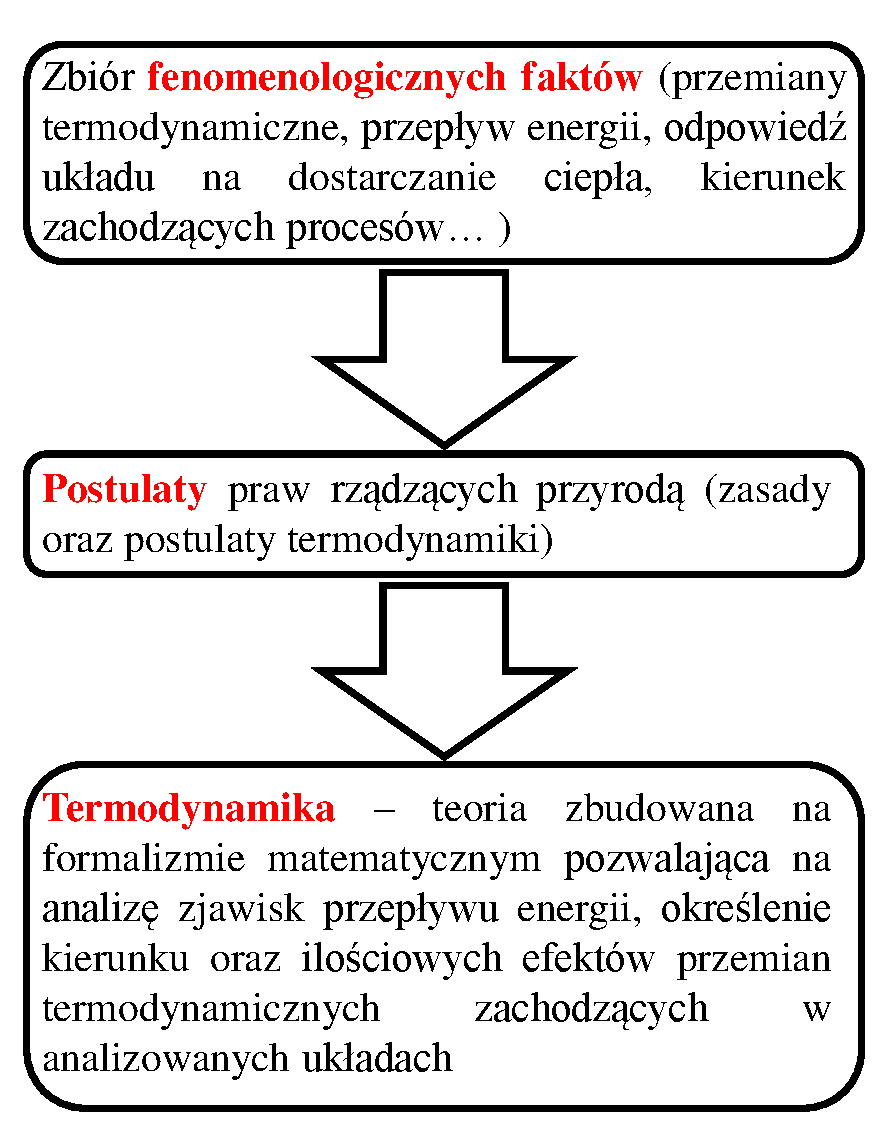
\includegraphics[width=6cm, clip]{rysunki/1_sch_td}
\caption{Schemat struktury termodynamiki.}
\label{1_sch_td}
\end{figure}
%
\subsection{Układ termodynamiczny} 
Układem termodynamicznym nazywamy wyodrębnioną część świata materialnego (masa, skład chemiczny itp.). Materia pozostała poza układem stanowi otoczenie, a granicę pomiędzy dwoma częściami stanowi brzeg układu. Przykładami układów termodynamicznych mogą być: wnętrze silnika, naczynie z gazem lub cieczą, w którym zachodzi jakaś interesująca przemiana, lub np. obszar całej elektrowni, dla którego określa się przepływy ciepła. Powyższa koncepcja została przedstawiona na Rysunku (\ref{2_uk_td}).\\
\\
Dzięki ograniczeniu danego zjawiska do układu można osobno rozpatrywać procesy wewnątrz układu i procesy wymiany energii między układem i otoczeniem. \\
W zależności od granicy, układy termodynamiczne można podzielić na: \\
• otwarte - wymienia z otoczeniem energię i masę, \\
• zamknięte - wymienia z otoczeniem energię, nie wymienia masy, \\
• izolowane - nie wymienia z otoczeniem ani energii ani masy. \\
%
\begin{figure}[h!]
\centering
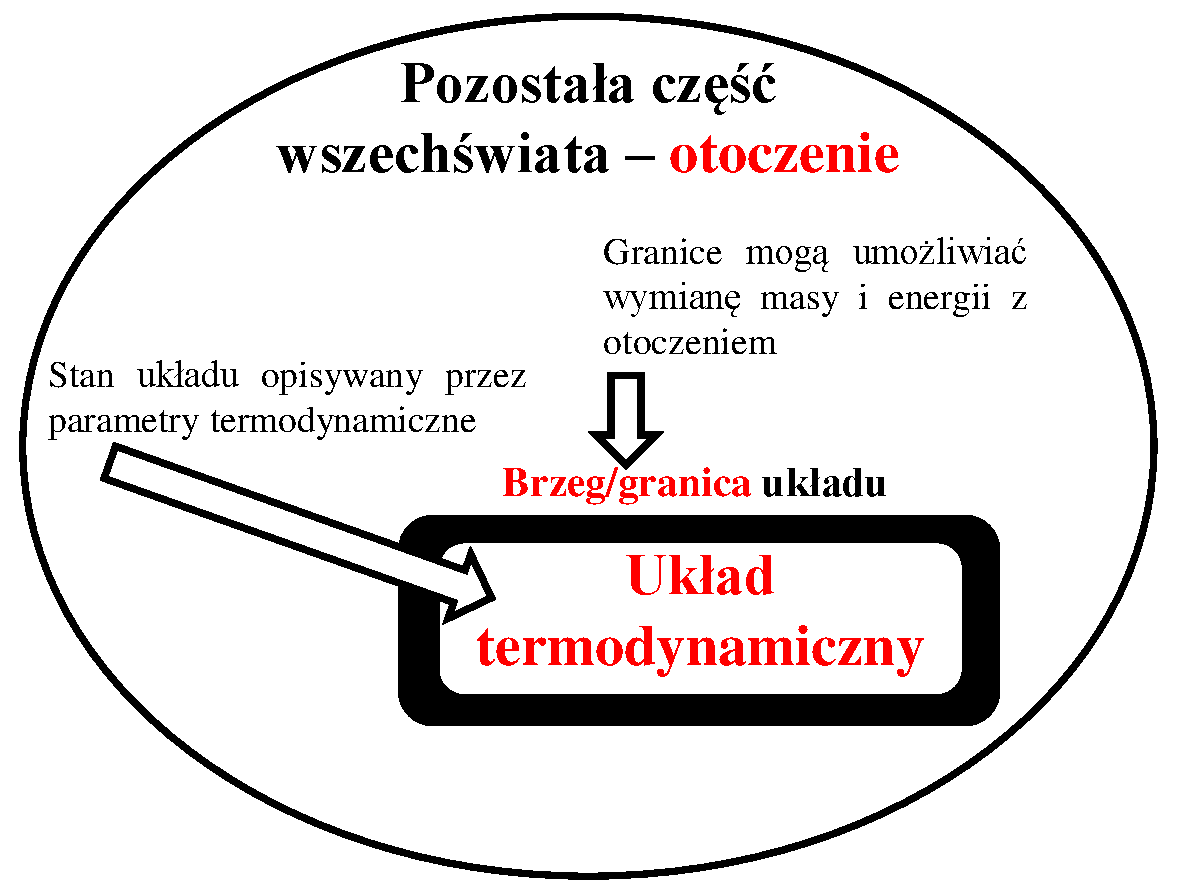
\includegraphics[width=10cm, clip]{rysunki/2_uk_td}
\caption{Koncepcja układu termodynamicznego.}
\label{2_uk_td}
\end{figure}
%
\subsection{Parametry opisujące stan układu} 
Przez parametry stanu należy rozumieć wielkości fizyczne opisujące stan układu termodynamicznego takie jak: temperatura $T$, ciśnienie $P$, objętość $V$, ilości (np. stężenia) poszczególnych substancji, liczba cząsteczek $N$, energia wewnętrzna $U$, entropia $S$, etc. \\
\\
Wielkości, które nie zależą od ilości substancji w układzie, to tzw. \textbf{parametry intensywne}, natomiast wielkości zależące od ilości substancji to \textbf{parametry ekstensywne}. \\
\\
Parametry stanu układu możemy podzielić na:\\
• \textbf{parametry intensywne} - ($P$, $T$, $\rho$) - niezależne od ilości materii w układzie\\
• \textbf{parametry ekstensywne} - ($V$, $N$, $U$, $S$) - addytywne, proporcjonalne do ilości materii w układzie. Iloraz dwóch wielkości ekstensywnych zawsze jest wielkością intensywną. \\
Wyjątki, które wychodzą poza ten podział, pojawiają się gdy – układ jest mały, istnieje niejednorodny potencjał zewnętrzny, istnieją oddziaływania dalekozasięgowe, geometria jest taka, że powierzchnia wpływa na własności całego układu.\\
\\
Parametry stanu układu można również podzielić na:\\
• \textbf{parametry wewnętrzne} – określone przez stan wydzielonego układu,\\
• \textbf{parametry zewnętrzne} – zadane.\\
%
\subsection{Granica termodynamiczna} 
Zgodność przewidywań termodynamicznych z doświadczeniem jest spełniona w tak zwanej granicy termodynamicznej, zdefiniowanej następująco (w odniesieniu do wiedzy na temat atomowej budowy materii): $N \rightarrow \infty, V \rightarrow \infty, \frac{N}{V}=n=const.$\\
Można powiedzieć, że układ spełniający tą granicę jest \textbf{translacyjnie niezmienniczy}.
Warto zauważyć, że gęstość $n$ jest \textbf{parametrem intensywnym}, jako iloraz dwóch parametrów ekstensywnych.
W świecie makroskopowym, za wygodną liczbę cząsteczek $N$ możemy przyjąć liczbę Avogadry, $N_A=6,22 \cdot 10^{23}$, natomiast za $V$, objętość jednego mola gazu w warunkach normalnych, $V_A=22,4 dm^3$.
\subsection{Układ modelowy - gaz doskonały} 
Gaz doskonały to najprostszy, wyidealizowany układ termodynamiczny, który jest granicznym przypadkiem dowolnego gazu o niskiej gęstości i wysokiej temperaturze. Stan takiego układu może być w pełni opisany za pomocą parametrów $P$, $V$, i $T$. Okazuje się, że te parametry są powiązane wzajemnie pewną matematyczną zależnością - zmiana wartości jednego z nich wpływa na wartość pozostałych.\\
\\
Empiryczne obserwacje poczynione przez:\\
• Boyle’a-Mariotte’a – przemiana izotermiczna ($PV=const.$),\\
• Charlsa – przemiana izochoryczna ($P/T=const.$),\\
• Gay-Lussaca – przemiana izobaryczna ($V/T=const.$).\\
pozwoliły na sformułowanie przez Clapeyrona równania stanu gazu doskonałego,
\begin{equation}
PV=nRT,
\end{equation}
gdzie:
$P$ – ciśnienie, $V$ – objętość, $n$ – liczba moli gazu, 
$R$ – uniwersalna stała gazowa, $T$ – temperatura układu.\\
\\
Zauważono również, że zmiana wartości parametrów termodynamicznych układu znajdującego się w równowadze wiąże się z wymianą energii między układem a otoczeniem w postaci ciepła lub pracy.
%
\subsection{Zasady termodynamiki} 
Zasady termodynamiki to prawa dotyczące pomiaru, wartości oraz kierunku przepływu energii. Stanowią podstawowe i najczęściej omawiane sformułowanie termodynamiki\\
\\
\textbf{Zerowa zasada termodynamiki} opiera się na założeniu istnienia równowagi termodynamicznej. \textbf{Równowagą termodynamiczną} nazywamy sytuację, w której między dwoma ciałami będącymi w kontakcie termicznym, nie dochodzi do wymiany energii (w postaci ciepła lub pracy), co za tym idzie, wszystkie parametry opisujące układ przybierają stałe wartości (niezmieniające się w czasie). Wartości tych parametrów informują nas o aktualnej własnej energii wewnętrznej układu, której miarę nazywamy \textbf{temperaturą}. 
Treść zerowej zasady termodynamiki jest następująca:
%
\begin{center}
\textit{Jeżeli ciało A i B znajdują się w równowadze termodynamicznej z ciałem C, to są one również w stanie równowagi termodynamicznej ze sobą nawzajem.}
\end{center}
Powyższą zasadę ilustruje Rysunek (\ref{3_ZZT}).
\begin{figure}[h!]
\centering
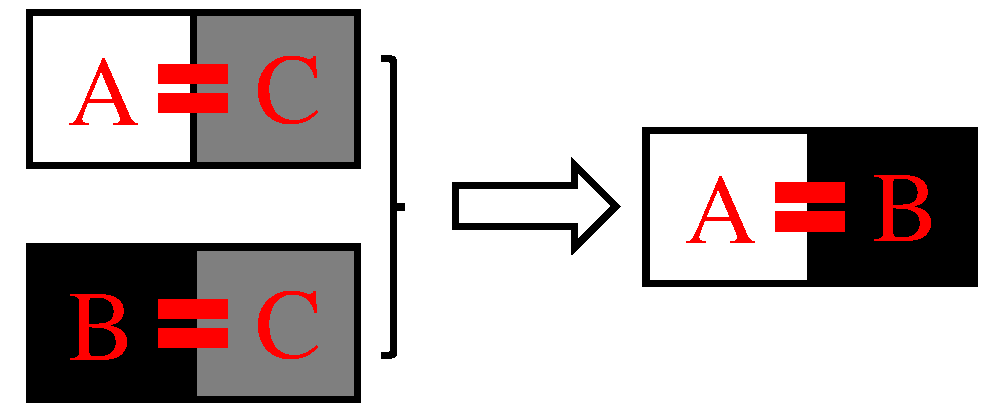
\includegraphics[width=8cm, clip]{rysunki/3_ZZT}
\caption{Ilustracja Zerowej Zasady Termodynamiki. Równowaga termodynamiczna ciał \textit{A} z \textit{C} oraz \textit{B} z \textit{C} oznacza równowagę między ciałami \textit{A} i \textit{B}.}
\label{3_ZZT}
\end{figure}
%
\\
Temperatura jest jedynym intensywnym parametrem określającym równowagę diatermalnych (będących w kontakcie cieplnym) układów termodynamicznych. Pomiar temperatury jest możliwy, ponieważ każdy układ posiada właściwości związane ze stanem termodynamicznym (objętość, długość, opór, przewodnictwo, ciśnienie, etc.). 
\textbf{Termometrem} nazywamy urządzenie, którego wskazanie zmienia się wraz z doprowadzeniem do niego energii cieplnej. Kalibracja zaproponowanego urządzenia polega na odniesieniu się do powtarzalnych zjawisk zależnych od temperatury (np. zmiany stanów skupienia wody, które stanowią podstawę temperaturowej skali Celsjusza).
\\
\\
\textbf{Pierwsza zasada termodynamiki} stanowi zasadę zachowania energii w procesach termodynamicznych. Procesem termodynamicznym może być wymiana ciepła między układem a otoczeniem lub wykonanie pracy. Przez \textbf{pracę} będziemy rozumieć zmianę objętości układu przy stałym ciśnieniu $\delta W= -P \delta V$. Przez \textbf{ciśnienie} z kolei wartość działającej siły na zadaną powierzchnię $P=F/N$.\\
W konsekwencji procesu termodynamicznego zmianie ulegają parametry opisujące stan układu. Taką sytuację ilustruje Rysunek (\ref{4_PZT}). 
%
\begin{figure}[h!]
\centering
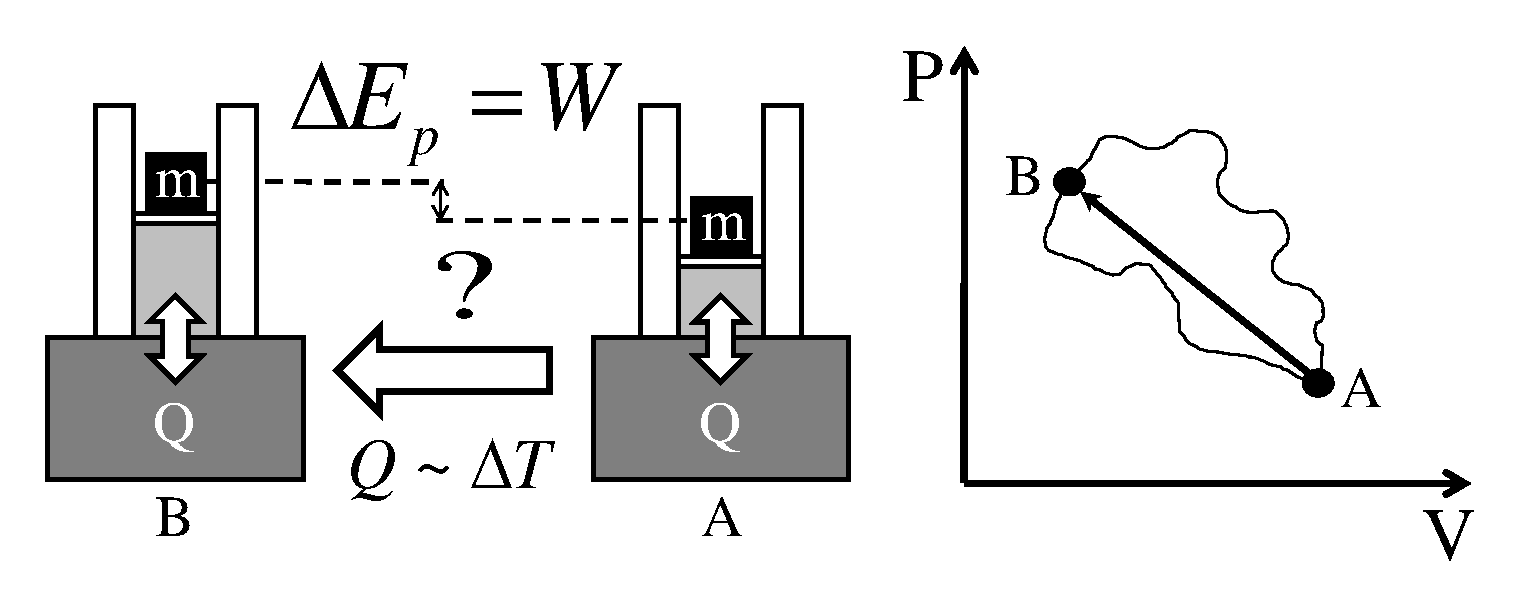
\includegraphics[width=10cm, clip]{rysunki/4_PZT}
\caption{Ilustracja Pierwszej Zasady Termodynamiki. Układem jest gaz zamknięty ruchomym tłokiem w cylindrze. Cylinder jest w kontakcie cieplnym z termostatem. Układ pobiera ciepło z termostatu. Ogrzewany gaz wykonuje pracę związaną z podniesieniem odważnika umieszczonego na tłoku o masie $m$.}
\label{4_PZT}
\end{figure}
%
Początkowy stan układu można przedstawić na płaszczyźnie $P-V$ jako punkt $A$. Na drodze procesu termodynamicznego (wymiana ciepła $Q$, wykonanie pracy $W$), wartości parametrów opisujących stan układu zmieniają się. Końcowy stan układu reprezentuje punkt $B$. Przejście $A-B$ może odbyć się różnymi drogami. Dla każdej z tych dróg, przez układ przepływa inna wartość ciepła i wykonywana jest (lub dostarczana) inna praca, ale w każdym z przypadków efekt jest ten sam – układ przechodzi z punktu $A$ do punktu $B$. Okazuje się, że w każdym z tych przypadków różnica $Q-W$ ma stałą wartość - nie zależy od drogi po której odbywa się proces. W związku z tym różnica $Q-W$ musi odpowiadać zmianie pewnej wielkości opisującej układ. Wielkość tą nazywamy \textbf{energią wewnętrzną} \textit{U}, natomiast jej zmianę zapisujemy:
\begin{equation}
\Delta U=\Delta Q- \Delta W ~~ lub ~~ d U = \delta Q - \delta W,
\end{equation}
Pierwszą zasadę termodynamiki można ująć w następujący sposób:
%
\begin{center}
\textit{Energia wewnętrzna układu wzrasta o $dU$ gdy pobiera on ciepło $\delta Q$ i maleje gdy wykonuje pracę $\delta W$. Przy czym $\delta Q$ i $\delta W$, w przeciwieństwie do $dU$, nie stanowią różniczek zupełnych, ponieważ nie istnieją funkcje $Q(p,V)$, $W(p,V)$, \\ które zależałyby tylko od stanu układu (tzn. nie określają stanu układu). 
}
\end{center}
Pośród wielu procesów termodynamicznych można wyróżnić przypadki szczególne, dla których pierwsza zasada termodynamiki przyjmuje uproszczoną postać:\\
• Przemiana izotermiczna, $T=const, ~~ dU=\delta Q- \delta W$, \\
• Przemiana adiabatyczna, $\delta Q=0, ~~ dU=-\delta W$, \\
• Przemiana przy stałej objętości, $V=const, ~~ dU=\delta Q$, \\
• Proces cykliczny, $dU=0, ~~ \delta W=\delta Q$, \\
• Rozprężanie swobodne, $\delta Q=\delta W=dU=0$, (proces nieustalony – można wyznaczyć tylko stan początkowy i końcowy, ale nie można wyznaczyć drogi po której się odbywa) \\
\\
\textbf{Procesy nieodwracalne} - przemianę jednokierunkową nazywamy nieodwracalną, jeśli nie można odwrócić jej kierunku za pomocą niewielkich zmian w otoczeniu. \\
Większość procesów fizycznych jest nieodwracalna. Przykładami mogą być spadające ciała, które po upadku wytrącają swój pęd zwiększając swoją energię wewnętrzną. Warto zauważyć, że procesy nieodwracalne zachodzą w ściśle określonym kierunku, którego nie można wyjaśnić na gruncie pierwszej zasady termodynamiki. Dla przykładu, pierwsza zasada termodynamiki stawia na równi sytuacje w których upadające z pewnej wysokości ciało, po zderzeniu z powierzchnią ziemi zwiększa swoją energię wewnętrzną oraz sytuację w której ciało kosztem własnej energii wewnętrznej samoistnie uniosłoby się na zadaną wysokość. Bilans energetyczny obu procesów jest taki sam. Mimo tego, nie obserwujemy samoistnych procesów w których obiekty kosztem energii wewnętrznej wykonywałyby pracę związaną z podnoszeniem na zadaną wysokość. Można powiedzieć, że pierwsza zasada termodynamiki, a tym samym zasada zachowania energii nie determinuje kierunku zachodzenia procesów fizycznych. Ta fenomenologiczna obserwacja każe sądzić, że istnieje inny potencjał termodynamiczny, który wyznacza kierunek przebiegu procesów samorzutnych. Ten potencjał to \textbf{entropia} $S$, a kierunek zachodzących procesów określa jej wzrost. Pojęcie entropii pozwala na sformułowanie drugiej zasady termodynamiki.\\
\\
\textbf{Perpetuum mobile I rodzaju} – maszyna która wykonuje więcej pracy niż pobiera energii – sprzeczna z zasadą zachowania energii (w tym również z pierwszą zasadą termodynamiki).\\
\\
\textbf{Perpetuum mobile II rodzaju} – maszyna, która przemienia na użyteczną pracę bez jakichkolwiek strat całe pobrane ciepło – pomija zamianę części ciepła na zmianę entropii układu. Niezgodna z drugą zasadą termodynamiki. \\
\\
\textbf{Druga zasada termodynamiki} może być sformułowana na wiele równoważnych sposobów:\\
\textit{• Postulat Clausiusa – ciepło nie może samorzutnie przepływać od ciała o temperaturze niższej do ciała o temperaturze wyższej.}\\
\textit{• Postulat Kelvina – nie jest możliwy proces, którego jedynym skutkiem byłoby pobranie pewnej ilości ciepła ze zbiornika i zamiana go w równoważną ilość pracy.}\\
\textit{• Spontaniczny przekaz ciepła może odbywać się tylko od ciała cieplejszego do zimniejszego.}\\
\textit{• Nie można bez wkładu pracy przesyłać energii termicznej między ciałami mającymi tą samą temperaturę. Nie możliwe jest istnienie perpetuum mobile II rodzaju.}\\
%
\\
Powyższe postulaty pozwalają wysunąć wniosek, że kierunek przebiegu samorzutnych procesów nieodwracalnych jest determinowany przez pewien potencjał – funkcję stanu układu (entropię). Każdy proces samorzutny przebiega w takim kierunku, aby wartość tej funkcji rosła lub ją zachowywała (jeśli proces jest odwracalny). Dostarczenie do układu ciepła powoduje (oprócz zmiany energii wewnętrznej i wykonania pracy), zmianę entropii. Korzystając z pojęcia entropii, drugą zasadę termodynamiki można sformułować następująco:
%
\begin{center}
\textit{W układzie izolowanym termodynamicznie, \\ w dowolnym procesie 
entropia nigdy nie maleje.}
\end{center}
%
\textbf{Entropia} stanowi funkcję stanu, tzn. jej wartość zależy od stanu początkowego i końcowego układu, nie zależy zaś od drogi po której odbył się proces.
Aby wyznaczyć zmianę entropii w przemianie nieodwracalnej w układzie zamkniętym, należy zastąpić tą przemianę dowolną przemianą odwracalną, która ma ten sam stan początkowy i końcowy. Dla przemiany odwracalnej entropię obliczymy jako:
%
\begin{equation}
\Delta S=\int_{A}^{B} \frac{\delta Q}{T}
\end{equation}
To, że entropia istotnie jest funkcją stanu, możemy wnioskować jedynie dzięki doświadczeniu, jednak w szczególnym przypadku jakim jest gaz doskonały można tego dowieść teoretycznie. Dla gazu doskonałego, pierwsza zasada termodynamiki przyjmuje postać $dU=\delta Q - \delta W$, stąd $\delta Q = PdV + nC_V dT$.\\ Podstawiając za $P=\frac{nRT}{V}$ oraz dzieląc obustronnie przez $T$, otrzymujemy \\ $\frac{\delta Q}{T}=nR \frac{dV}{V}+nC_V \frac{dT}{T}$. Całkując obustronnie otrzymane wyrażenie, mamy \\ $\Delta S=nR \int_{A}^{B} \frac{dV}{V} +nC_V \int_{A}^{B} \frac{dT}{T}$, stąd $\Delta S = nR ln \left( \frac{V_B}{V_A} \right) + nC_V ln \left( \frac{T_B}{T_A} \right)$.
%
\\
\\
\textbf{Trzecia zasada termodynamiki} (zasada Nernsta) głosi, że zmniejszanie entropii wymaga coraz większego nakładu pracy, co wiąże się z asymptotycznym dążeniem do najniższej możliwej temperatury. Może być sformułowana jako postulat: \\
\\
\textit{Nie można za pomocą skończonej liczby kroków uzyskać temperatury zera bezwzględnego (zero kelwinów), jeżeli za punkt wyjścia obierzemy niezerową temperaturę bezwzględną.}\\
\\
Równoważne sformułowanie trzeciej zasady termodynamiki brzmi: \\
\\
\textit{Entropia układów tworzących doskonałe kryształy dąży do 0 gdy temperatura dąży do 0 K.}
\\
\subsection{Callenowskie sformułowanie termodynamiki} 
Postulaty Callena stanowią alternatywne sformułowanie termodynamiki.\\
\\
\textbf{Postulat I - istnienie stanu równowagi}
%
\begin{center}
\textit{Istnieją szczególne stany układu termodynamicznego, zwane stanami równowagi, które makroskopowo są całkowicie scharakteryzowane \\ przez wielkości ekstensywne (U, V, N, etc.)}
\end{center}
%
Istnienie stanu równowagi termodynamicznej daje możliwość pomiaru wszelkich parametrów układu. Termodynamika rozważa układy statyczne, bądź kwazistatyczne, natomiast funkcje stanu nie zależą od drogi procesu, ale od wartości początkowych i końcowych parametrów opisujących układ. Można powiedzieć, że stan równowagi termodynamicznej to sytuacja w której parametry opisujące układ nie ulegają zmianie a funkcje stanu (np. energia i entropia) posiadają ustalone (ekstremalne) wartości. Układ nie może spontanicznie (samorzutnie) zmieniać tego stanu.\\
\\
Podstawowym problemem termodynamiki jest ustalanie zmian funkcji i parametrów opisujących układ po przejściu z jednego stanu równowagi do drugiego. Wprowadzenie pojęcia równowagi nadaje sens tym rozważaniom.\\
\\
\textbf{Postulat II - istnienie entropii}
%
\begin{center}
\textit{Istnieje funkcja (zwana entropią) parametrów ekstensywnych zdefiniowana dla wszystkich stanów równowagowych. Te parametry przyjmują takie wartości aby entropia była maksymalna. Funkcja ta dostarcza nam wszelkich informacji na temat układu - stanowi relację fundamentalną.}
\end{center}
%
Zgodnie z II postulatem, entropia to relacja fundamentalna, którą można przedstawić jako funkcję wielkości ekstensywnych $S=S(U,V,N)$. Entropia jest postulowana tylko dla stanów równowagowych, czyli takich, dla których jej pochodna będzie się zerować, czyli $dS=0$.\\
\\
\textbf{Postulat III - addytywność i monotoniczność wzrostu entropii}
\begin{center}
\textit{Entropia układu termodynamicznego jest sumą entropii jego mikroskopowych części. Stanowi ona ciągłą, różniczkowalną i monotonicznie (zachowuje określony porządek zbiorów w całej dziedzinie) rosnącą  funkcją energii.}
\end{center}
Fakt, że entropia układu jest sumą entropii jego części nazywamy \textbf{addytywnością} i zapisujemy $S=\sum\limits_{k} S_k(U_k, V_k, N_k)$. \\
Dla układu prostego entropia jest jednorodną funkcją pierwszego rzędu parametrów ekstensywnych, tzn. $S(\lambda U, \lambda V, \lambda N)=\lambda S(U, V, N)$. \\
Postulat monotoniczności implikuje $\left( \frac{\partial S}{\partial U} \right)_{V,N}>0$, co wprowadza zawsze dodatnią temperaturę $1/T >0$, tym samym pokrywa się z zerową zasadą termodynamiki.\\
Ciągłość, różniczkowalność, monotoniczność umożliwia przekształcenie funkcji entropii w funkcję energii (jednowartościową, ciągłą, różniczkowalną) zależną od $S, V, N_1,...N_r $. Daje to alternatywną postać relacji fundamentalnej (postać funkcji energii wewnętrznej), $S(U, V, N_1, ...) \rightarrow U(S, V, N_1,...)$. \\
\\
Wyznaczmy różniczkę nowozdefiniowanej funkcji U. \\
$dU=\left( \frac{\partial U}{\partial S} \right)_{V, N} dS + \left( \frac{\partial U}{\partial V} \right)_{S, N} dV + \left( \frac{\partial U}{\partial N} \right)_{S, V} dN$. \\
Pochodne energii wewnętrznej po wielkościach ekstensywnych dają w wyniku wielkości intensywne. Uwzględniając postać $U$, jako $U(S, V, N) = TS - PV - \mu N$, możemy nadać sens kolejnym pochodnym cząstkowym: $\left( \frac{\partial U}{\partial S} \right)_{N,V}=T$, $\left( \frac{\partial U}{\partial V} \right)_{S,N}=-P$, $\left( \frac{\partial U}{\partial N} \right)_{S,V}=\mu$. Podstawiając otrzymane związki do różniczki $dU$ otrzymujemy: $dU=TdS-PdV+\mu dN$ oraz $dU = \delta Q + \delta W$, a więc otrzymaliśmy z relacji fundamentalnej pierwszą i drugą zasadę termodynamiki. Znajomość relacji fundamentalnej pozwala nam wyznaczyć inne równania stanu, czyli relacje wyrażające parametry intensywne za pomocą niezależnych parametrów ekstensywnych $T=T(S, V, N), P=P(S, V, N), \mu = \mu(S, V, N)$.\\
\\
\textbf{Postulat IV - zerowanie entropii}
\begin{center}
\textit{Entropia każdego układu zeruje się w temperaturze 0K, \\ czyli wówczas gdy $\left( \frac{\partial U}{\partial S} \right)_{V, N_1,...,N_r}=0$
}
\end{center}
Postulat ten pokrywa się z trzecią zasadą termodynamiki.\\
\\
%\subsection{Właściwości entropii jako relacji fundamentalnej} 
%\markright{Właściwości entropii jako relacji fundamentalnej}
%Jeżeli relacja fundamentalna jest jednorodną funkcją pierwszego rzędu, to\\
%\textit{
%• Można przedstawić ją w wygodnej postaci nazywanej relacją Eulera \\
%• Musi istnieć związek pomiędzy parametrami intensywnymi (relacja Gibbsa-Duhema)\\
%}
%\\
%Jednorodność oraz pierwszorzędowość relacji fundamentalnej pozwala zapisać jej równanie w wygodnej formie nazywanej równaniem Eulera, oraz wyznaczyć relację wiążącą parametry intensywne – relacja Ginnsa-Duhema.
%Z definicji jednorodności i pierwszorzędowości: $U(\lambda S, \lambda V, \lambda N) = \lambda U(S, V, N)$. Różniczkując obustronnie uzyskane równanie po $\lambda$ oraz przyjmując $\lambda = 1$ otrzymujemy:
\subsection{Warunki równowagi termodynamicznej} 
Istnienie stanu równowagi zapewnia pierwszy postulat Callena. Każdy układ przejawia dążność do tego stanu, natomiast wiąże się z tym osiąganie wartości ekstremalnej przez relację fundamentalną, o czym mówi II postulat. Ponieważ zgodnie z II postulatem, parametry relacji fundamentalnej przyjmują takie wartości aby entropia była maksymalna, należy wnioskować, że \textbf{w stabilnym układzie entropia jest wklęsłą funkcją energii}.  
\subsection{Potencjały termodynamiczne} 
Proces termodynamiczny może być prowadzony w innych warunkach niż stałe $U, V, N$ (w tym przypadku, przejście ze stanu $P$ do $K$ we współrzędnych $(p, V)$ wiązało się z dostarczeniem lub odebraniem od układu $W$ i $Q$). Zmiana warunków realizacji procesu wiąże się ze zmianą sposobów na jakie układ może wymieniać energię z otoczeniem (np. $T=const$, $p=const$). Wówczas układ przyjmuje energię na inne sposoby (np. praca nieobjętościowa), natomiast różnica form energii dostarczonych i odebranych z układu na drodze $P-K$ ma inną wartość (niż $U$ w układzie $p-V$ przy wymianie $Q$, $W$), jednak nadal stanowi różniczkę zupełną (nie zależy od drogi prowadzenia procesu). W zależności od współrzędnych w których prowadzimy proces termodynamiczny oraz form wymiany energii z układem, otrzymujemy różne różniczki zupełne, które nazywamy też potencjałami termodynamicznymi. 
Formalny, matematyczny związek między poszczególnymi potencjałami związanymi z poszczególnymi układami współrzędnych termodynamicznych stanowi transformata Legendra. Do najważniejszych potencjałów termodynamicznych (z punktu widzenia zastosowań) należą:
\\
\\
\textbf{a) Energia swobodna Helmholtza F(T,V,N).} W termodynamice energia swobodna Helmholtza to funkcja stanu i potencjał termodynamiczny - odpowiada tej części energii wewnętrznej, która może być w danym procesie uwolniona na zewnątrz układu w formie pracy lub ciepła przy stałej temperaturze i objętości.\\
Jest to przydatna funkcja, w odróżnieniu od energii wewnętrznej, można ją łatwo wyznaczyć gdyż zależy w sposób naturalny od temperatury, objętości i liczby moli substancji, a parametry te można łatwo mierzyć. Funkcji tej używa się często przy złożonych procesach, w których przekazywanie energii odbywa się na kilka różnych sposobów (np:reakcja chemiczna połączona ze zmianą temperatury i ciśnienia).\\
\\
\textbf{b) Entalpia H(S,P,N).} Entalpia jest równa sumie energii wewnętrznej, czyli energii jaka jest potrzebna do utworzenia układu gdy jest on tworzony w otoczeniu próżni oraz iloczynu $pV$, który jest równy pracy jaką należy wykonać nad otoczeniem by w danych warunkach uzyskać miejsce na układ.\\
Wszystkie wielkości definiujące entalpię są funkcjami stanu, dlatego entalpia też jest funkcją stanu.\\
\\
\textbf{c) Entalpia swobodna Gibbsa G(T,P,N).} Entalpia swobodna w przemianach izotermiczno-izobarycznych ($dp=0$, $dT=0$) jest równa maksymalnej pracy nieobjętościowej , np. elektrycznej, którą można uzyskać w takiej przemianie. Dlatego odgrywa dużą rolę w elektrochemii.\\
W procesach samorzutnych przebiegających pod stałym ciśnieniem oraz w stałej temperaturze entalpia swobodna nie wzrasta (maleje lub zachowuje wartość). Kryterium to jest często stosowane gdyż reakcje chemiczne oraz zmiany stanów skupienia przebiegają często przy stałym ciśnieniu a przy możliwej zmianie objętości. Reakcja zachodzi samorzutnie przy stałym ciśnieniu i określonej temperaturze, tylko gdy entalpia swobodna substratów jest nie mniejsza od entalpii swobodnej produktów.\\

\subsection{Przejścia fazowe} 
Jeśli kryteria stabilności nie są spełnione, w układzie zachodzi \textbf{przejście fazowe}. \\
\textbf{Fazą} nazywamy obszar w przestrzeni (fragment) substancji w którym wszystkie właściwości fizyczne i chemiczne są zasadniczo jednorodne. Przykładami takich właściwości mogą być gęstość, współczynnik załamania światła, skład chemiczny.\\
W czasie przejścia fazowego dochodzi do gwałtownej zmiany właściwości układu.
Przemianie fazowej często towarzyszy skokowa zmiana parametrów układu, np. gęstości substancji ulegającej przemianie, oraz wyzwolenie lub pochłonięcie ciepła – taką przemianę nazywamy "przemianą nieciągłą" lub "pierwszego rodzaju".\\
Z punktu widzenia potencjału termodynamicznego można powiedzieć, że w stanie równowagi, układ znajduje się w najkorzystniejszym minimum potencjału termodynamicznego. Układ może posiadać wiele minimów. Zmieniając zewnętrzne, zadawane parametry można zmienić pozycję tych minimów i przeprowadzić układ z jednego do drugiego. 
Przejście fazowe jest zawsze konsekwencją \textbf{niespełnienia kryteriów stabilności}. 
%Poniższy rysunek pokazuje potencjał Gibbsa pewnego układu dla różnych temperatur. Widać z niego, że poprzez zmianę parametrów %zewnętrznych minima zamieniają się pozycjami – pierwsze minimum się obniża, a drugie podwyższa. Temperatura T4 stanowi %temperaturę przejścia fazowego w której oba minima są równie korzystne.  
W czasie przejścia fazowego (np. cieczy w gaz) równanie stanu w każdej z tych faz jest regularną funkcją ciągłą o ciągłych pochodnych. Jednak w czasie przechodzenia z jednej fazy do drugiej zmienia się ona gwałtownie w inną regularną funkcję. Jest to \textbf{przejście fazowe nieciągłe}, dla którego pierwsza pochodna potencjału Gibbsa jest nieciągła na granicy pomiędzy fazami. Znane są również przykłady przejść w których funkcja $G$ w trakcie zmiany fazy jest ciągła i posiada ciągłe pochodne pierwszego rzędu (lub również wyższych rzędów). Takie przejścia nazywane są \textbf{przejściami nieciągłymi}. Podział przejść fazowych na ciągłe i nieciągłe stanowi podstawę \textbf{klasyfikacji przejść fazowych Landaua-Ginzburga}. 
\\
Przejścia fazowe można również podzielić ze względu na nieciągłość kolejnych pochodnych \textbf{potencjału chemicznego} $\mu$ (pochodna cząstkowa energii wewnętrznej po liczbie cząstek przy stałej objętości i entropii układu). W myśl tego podziału przemiana \textit{n-tego} rodzaju to taka, dla której najniższa nieciągła pochodna $\mu$ jest \textit{n-tą} pochodną potencjału chemicznego $\frac{\partial^n \mu}{\partial T^n}$. Przytoczony podział stanowi podstawę \textbf{klasyfikacji Ehrenfesta przejść fazowych}. 

\section{Elementy mechaniki klasycznej}
Mechanika klasyczna to dział fizyki, który zajmuje się głównie opisem ruchu i jego przyczyn oraz badaniem równowagi ciał materialnych. Dla symulacji MD jest to szczególnie istotny dział, ponieważ każdy element symulowanego układu musi spełniać prawa mechaniki. W tej części zostaną omówione najważniejsze pojęcia z zakresu mechaniki, które ułatwią czytelnikowi zromumienie języka i metod omawianych w dalszych częściach.
\subsection{Podstawowe pojęcia}
\textbf{Punkt materialny} to jedno z podstawowych pojęc mechaniki. Należy przez nie rozumieć ciało, którego rozmiary można pominąć przy opisie jego ruchu. 
Położenie punktu materialnego w przestrzeni jest określone przez jego \textbf{wektor wodzący} $\underline{r}$, którego składowe są współrzędnymi kartezjańskimi $x$, $y$, $z$ punktu materialnego. Kolejne pochodne wektora położenia po czasie to odpowiednio \textbf{prędkość} i \textbf{przyspieszenie} $\underline{v}=\frac{d \underline{r}}{dt}$, $\underline{a}=\frac{d^2 \underline{r}}{dt^2}$. Położenie $N$ punktów materialnych opisuje $N$ wektorów wodzących, które można przedstawić w postaci $3N$ współrzędnych. Liczbę niezależnych wielkości koniecznych do opisu położenia układu nazywa się \textbf{liczbą stopni swobody}. Położenie nie musi być określane za pomocą współrzędnych kartezjańskich. W wielu zagadnieniach wybór innego układu współrzędnych znacznie upraszcza opis zjawiska ruchu. Z tego powodu będziemy posługiwać się pojęciem \textbf{współrzędnych uogólnionych}, czyli zestawu $s$ dowolnych wielkości $q_1, q_2, q_3...$ który jednoznacznie opisuje położenie układu. Odpowiednio pochodne tych wielkości będą \textbf{prędkościami uogólnionymi} układu. Mechaniczny stan punktu materialnego (lub układu punktów) jest w pełni opisany przez zestaw jego współrzędnych i prędkości (pędów) uogólnionych. Zestaw współrzędnych i prędkości uogólnionych można przedstawić w postaci punktu w \textbf{przestrzeni fazowej} $\Gamma$ czyli przestrzeni możliwych położeń i prędkości (pędów). Punkt opisujący stan układu będziemy nazywać \textbf{punktem fazowym}, którego znajomość w zasadzie pozwala przewidzieć dalszy ruch układu.   
\subsection{Lagranżowskie sformułowanie mechaniki}
Najbardziej ogólnym sformułowaniem mechaniki jest \textbf{zasada najmniejszego działania}. Mówi ona, że każdy układ mechaniczny jest w pełni opisany przez funkcję jego położeń i prędkości uogólnionych oraz czasu,
\begin{equation}
L=f(q_1, g_2,...,\dot{q}_1, \dot{q}_2,...,t),
\end{equation} 
którą będziemy oznaczać jako $L(q,\dot{q},t)$. Ruch układu spełnia następujący warunek. Niech w chwilach $t_1$ i $t_2$ stan układu będzie opisany przez zbiory wartości odpowiednio $q^{(1)}$ i $q^{(2)}$. Wówczas między tymi położeniami układ porusza się tak, że całka 
\begin{equation}
S=\int\limits_{t_1}^{t_2}L(q, \dot{q}, t) dt
\end{equation} 
przyjmuje najmniejszą możliwą wartość. Funkcję $L$ będziemy nazywać \textbf{funkcją Lagrange'a} danego układu, a całkę $S$ \textbf{działaniem} tego układu. Powyższe sformułowanie to tzw. \textbf{zasada najmniejszego działania}. Warto zauważyć, że funkcja Lagrange'a zależy tylko od $q$ i $\dot{q}$ a nie zależy od wyższych pochodnych. Jest formalnym odpowiednikiem stwierdzenia, że stan mechaniczny układu jest jednoznacznie określony przez współrzędne i prędkości. \\
Żądanie minimalizacji wartości całki $S$ prowadzi do uzyskania rozwiązania, które dla układu o $N$ stopniach swobody przyjmuje postać układu równań
\begin{equation}
\frac{d}{dt}\frac{\partial L}{\partial \dot{q}_i}-\frac{\partial L}{\partial {q}_i}=0, ~~~~~~ (i=1,2,...N).
\label{eq:rownanie_lagrangea}
\end{equation} 
Równania te są szukanymi równaniami różniczkowymi (minimalizują funkcjonał $S$) i noszą nazwę \textbf{równań Lagrange'a}. Do całkowitego określenia ruchu układu mechanicznego, konieczna jest znajomość warunków początkowych opisujących stan układu w ustalonej chwili czasu. Może to być zestaw początkowych współrzędnych i prędkości. W odniesieniu do dynamiki molekularnej, szczególnie istotne jest zagadnienie \textbf{funkcji Lagrange'a układu oddziałujących punktów materialnych}. Zakładamy, że punkty materialne oddziałują ze sobą i nie oddziałują z żadnym zewnętrznym ciałem. Taki układ będziemy nazywać układem \textbf{odosobnionym}. Okazuje się, że oddziaływanie między punktami można uwzględnić dodając do funkcji Lagrange'a punktów nieoddziałujących pewną funkcję współrzędnych
\begin{equation}
L=\sum\limits_{i} \frac{m_i v_i^2}{2} - U(\underline{r}_1, \underline{r}_2, ...)=T-U,
\end{equation}
gdzie $\underline{r}_i$ to wektor położenia $i$-tego punktu. Funkcję $T = \sum\limits_{i} \frac{m_i v_i^2}{2}$ będziemy nazywać \textbf{energią kinetyczną}, natomiast funkcja $U(\underline{r}_1, \underline{r}_2, ...)$ zależy od charakteru oddziaływania i będziemy ją nazywać \textbf{energią potencjalną} układu.\\
Podstawiając uzyskaną postać funkcji $L$ do równania \ref{eq:rownanie_lagrangea} otrzymujemy różniczkowe równania drugiego rzędu
\begin{equation}
m_i \frac{d \underline{v}_i}{dt}=-\frac{\partial U}{\partial \underline{r}_i},
\end{equation}
które w tej postaci są nazywane \textbf{równaniami Newtona}, a wektor znajdujący się po prawej stronie $\underline{F}_i = -\frac{\partial U}{\partial \underline{r}_i}$ nazywa się \textbf{siłą} działającą na $i$-ty punkt. Równania Newtona są podstawą mechaniki układu oddziałujących cząstek.
\subsection{Prawa zachowania}
W czasie ruchu, stan układu jest jednoznacznie opisany przez $2s$ zmiennych w czasie wielkości $q_i$ oraz $\dot{q}_i$, gdzie $(i=1,2,...,s)$. Okazuje się jednak, że istnieją funkcje tych wielkości, które zachowują stałą wartość w czasie, która zależy wyłącznie od warunków początkowych. Takie funkcje nazywa się \textbf{całkami ruchu}. Dla odosobnionego układu mechanicznego o $s$ stopniach swobody, liczba niezależnych całek ruchu wynosi $2s-1$. Jednak nie wszystkie całki ruchu spełniają równie ważną rolę. Szczególnie interesujące i istotne dla symulacji Dynamiki Molekularnej są całki, których stałość wiąże się z podstawowymi własnościami czasu i przestrzeni (jednorodność i izotropowość). Wielkości odpowiadające tym całką mają dodatkową własność \textbf{addytywności} - wartość dla układu składającego się z nieoddziałujących części jest równa sumie odpowiednich wartości dla każdej takiej części. 
\\
\\
\textbf{ENERGIA}\\
\\
Rozważmy najpierw \textbf{zasadę zachowania energii}, która wiąże się z \textbf{jednorodnością czasu}. Przez jednorodność czasu należy rozumieć brak jawnej zależności funkcji Lagrange'a układu odosobnionego od czasu. Wówczas funkcję $L$ możemy zapisać
\begin{equation}
\frac{dL}{dt}=\sum \limits_{i} \frac{\partial L}{\partial q_i} \dot{q}_i+\sum \limits_{i} \frac{\partial L}{\partial \dot{q}_i}\ddot{q}_i
\end{equation}  
(ponieważ $L$ nie zależy jawnie od czasu, po prawej stronie równania pomijamy człon $\partial L / \partial t$). %
Zgodnie z równaniem Lagrange'a, możemy zastąpić pochodną $\frac{\partial L}{\partial q_i}$ na $\frac{d}{dt} \frac{\partial L}{\partial \dot{q}_i}$. Wówczas otrzymujemy
\begin{equation}
\frac{d}{dt}\left( \sum \limits_{i} \dot{q}_i \frac{\partial L}{\partial \dot{q}_i} -L \right) =0,
\end{equation}
skąd widać, że wielkość
\begin{equation}
\sum \limits_{i} \dot{q}_i \frac{\partial L}{\partial \dot{q}_i} -L=const
\end{equation}
jest zachowana w czasie. Tą wielkość będziemy nazywać \textbf{energią} układu. Zasada zachowania energii jest spełniona nie tylko dla układu odosobnionego ale dla każdego układu, którego funkcja Lagrange'a nie zależy jawnie od czasu. Układy mechaniczne, których energia jest zachowana nazywa się często \textbf{układami zachowawczymi}.
\\
\\
\textbf{PĘD}\\
\\
Kolejna zasada zachowania jest konsekwencją \textbf{jednorodności przestrzeni}. Przez jednorodność przestrzeni należy rozumieć (w odniesieniu do układu odosobnionego) niezależność własności mechanicznych układu przy dowolnym przesunięciu całego układu w przestrzeni. Rozpatrzmy nieskończenie małe, równoległe przesunięcie układu o odcinek $\epsilon$. Takie przesunięcie nie spowoduje zmiany prędkości cząstek. Funkcja Lagrange'a zmienia się o wielkość 
\begin{equation}
\delta L=\sum \limits_{i} \frac{\partial L}{\partial \underline{r}_i } \delta \underline{r}_i = \epsilon \sum \limits_{i} \frac{\partial L}{\partial \underline{r}_i},
\end{equation}
gdzie sumowanie odbywa się po wszystkich cząstkach układu. Ze względu na dowolność $\epsilon$ warunek $\delta L =0$ jest równoważny warunkowi
\begin{equation}
\sum \limits_{i} \frac{\partial L}{\partial \underline{r}_i}=0,
\label{eq:3ZDNLagranz}
\end{equation}  
wówczas w oparciu o równanie Lagrange'a otrzymujemy
\begin{equation}
\sum \limits_{i} \frac{d}{dt} \frac{\partial L}{\partial \underline{v}_i} = \frac{d}{dt} \cdot \sum \frac{\partial L}{\partial \underline{v}_i}=0,
\end{equation}
co pozwala wnioskować, że w odosobnionym układzie mechanicznym wielkość wektorowa
\begin{equation}
\underline{P}=\sum \limits_{i} \frac{\partial L}{\partial \underline{v}_i} = \sum \limits_{i} m_i \underline{v}_i
\end{equation} 
jest stała w czasie. Wektor $\underline{P}$ będziemy nazywać \textbf{pędem układu}. Pęd jest wielkością addytywną i w odróżnieniu od energii, pęd ukłądu jest równy sumie pędów składników.  
\\
Zasada zachowania wszystkich składowych wektora pędu jest słuszna tylko w sytuacji, jeżeli na układ nie działa żadne pole zewnętrzne. Jednak poszczególne składowe pędu mogą być zachowane również w obecności pola, jeśli energia potencjalna układu w tym polu nie zależy od rozważanej współrzędnej. Warto zauważyć, że z warunku \ref{eq:3ZDNLagranz} wypływa również tzw. \textbf{III zasada dynamiki Newtona}. $\frac{\partial L}{\partial \underline{r}_i}=-\frac{\partial U}{\partial \underline{r}_i}$. Stąd $\sum \limits_{i} \frac{\partial L}{\partial \underline{r}_i}=\sum \limits_{i} \underline{F}_i = 0,$ co stanowi treść trzeciej zasady dynamiki Newtona dla układów odosobnionych.
\\
\\
\textbf{ŚRODEK MASY}\\ 
\\
Zasada zachowania pędu ma dodatkową konsekwencję. Okazuje się, że zawsze istnieje taki układ odniesienia, w którym całkowity pęd układu jest równy zeru. Prędkość tego układu można wyrazić jako
\begin{equation}
\underline{V}=\frac{\underline{P}}{\sum \limits_{i} m_i}=\frac{\sum m_i \underline{v_i}}{\sum m_i}
\end{equation} 
Jeżeli całkowity pęd układu mechanicznego jest równy zeru, to znaczy, że układ spoczywa względem odpowiedniego punktu odniesienia. W ten sposób zasada zachowania pędu pozwala zdefiniować pojęcie \textbf{spoczynku}. Można przyjąć, że prędkość układu jako całości jest prędkością przemieszczenia w przestrzeni punktu, którego wektor wodzący wyraża wzór
\begin{equation}
\underline{R}=\frac{\sum m_i \underline{r}_i}{\sum{m_i}}.
\end{equation}
Taki punkt nazywać będziemy \textbf{środkiem masy układu}. Podsumowując, konsekwencją zachowania pędu układu odosobnionego jest ruch jednostajny jego środka masy.W szczególnym przypadku, gdy pęd całkowity układu jest równy zeru, środek masy pozostaje nieruchomy.
\\
\\
\textbf{MOMENT PĘDU}\\
\\
Kolejna zasada zachowania wiąże się z \textbf{izotropowością przestrzeni}. Przez izotropowość przestrzeni należy rozumieć niezależność własności mechanicznych układu od dowolnego obrotu układu jako całości. \\
Rozważmy  obrót układu o nieskończenie mały kąt reprezentowany przez wektor o wartości $\delta \varphi$. Wówczas zmiana wektora wodzącego układu wyniesie
\begin{equation}
\delta \underline{r} = \delta \underline{\varphi} \times \underline{r},
\end{equation}
a przyrost prędkości
\begin{equation}
\delta \underline{v}=\delta \underline{\varphi} \times \underline{v}.
\end{equation}
Podstawiając powyższe związki do warunku na niezmienniczość funkcji Lagrange'a przy obrocie, otrzymujemy
\begin{equation}
\delta L = \sum \limits_{i} \left( \frac{\partial L}{\partial \underline{r}_i} \delta \underline{r}_i + \frac{\partial L}{\partial \underline{v}_i} \delta \underline{v}_i \right)=0.
\end{equation}
Korzystając ze wcześniejszych definicji, możemy podstawić $\frac{\partial L}{\partial \underline{v}_i}=\underline{p}_i$, oraz $ \frac{\partial L}{\partial \underline{r}_i} = \dot{\underline{p}}_i$. Wówczas po przekształceniach (zmiana kolejności czynników, wyłączenie przed nawias $\delta \underline{\varphi}$) otrzymujemy
\begin{equation}
\delta \underline{\varphi} \frac{d}{dt}\sum \limits_{i} \underline{r}_i \times \underline{p}_i =0,
\end{equation}
co wobec dowolności $\delta \underline{\varphi}$ daje
\begin{equation}
\frac{d}{dt}\sum \limits_{i} \underline{r}_i \times \underline{p}_i =0.
\end{equation}
Powyższe równanie pozwala stwierdzić, że dla odosobnionego układu mechanicznego wielkość wektorowa $\underline{M}=\sum \limits_{i} \underline{r}_i \times \underline{p}_i$ jest zachowana w czasie. Wielkość wektorową $\underline{M}$ będziemy nazywać \textbf{momentem pędu} układu. Podobnie jak pęd, moment pędu jest wielkością addytywną i nie zależy od oddziaływania pomięczy cząstkami.
\\
\subsection{Hamiltonowskie sformułowanie mechaniki}
Formułowanie praw mechaniki i wyznaczanie równań ruchu za pomocą funkcji Lagrange'a opiera się na zestawie współrzędnych i prędkości uogólnionych. Nie jest to jedyne możliwe podejście. Równoważny opis może być oparty na zestawie uogólnionych współrzędnych i pędów. Przejście od jednego zbioru niezależnych zmiennych do innego zbioru można przeprowadzić przekształceniem matematycznym nazywanym transformatą Legendre'a. Wykonując transformację Legendre'a na funkcji Legandre'a (opartej na uogólnionych współrzędnych i prędkościach) otrzymujemy nową funkcję, zależną od uogólnionych współrzędnych i pędów
\begin{equation}
H(p,q,t)=\sum \limits_{i} p_i \dot{q}_i - L,
\end{equation}
którą będziemy nazywać \textbf{funkcją Hamiltona}. W oparciu o funkcję Hamiltona, równania ruchu przyjmują postać:
\begin{equation}
\dot{q}_i = \frac{\partial H}{\partial p_i}, ~~~~ \dot{p}_i=-\frac{\partial H}{\partial q_i}.
\label{eq:RownHam}
\end{equation}
\\
Powyższe równania są szukanymi równaniami ruchu w zmiennych $p, q$ i są nazywane \textbf{równaniami Hamiltona}. Dają one układ $2s$ równań różniczkowych pierwszego rzędu na $2s$ niewiadomych funkcji $q(t)$ i $p(t)$. Układ ten zastępuje układ $s$ równań drugiego rzędu w formalizmie Lagrange'a. Z powodu symetrii i formalnej prostoty, równania \ref{eq:RownHam} nazywa się \textbf{równaniami kanonicznymi}.
Zupełna pochodna funkcji Hamiltona względem czasu ma postać
\begin{equation}
\frac{dH}{dt}=\frac{\partial H}{\partial t} + \sum \frac{\partial H}{\partial q_i} \dot{q}_i + \sum \frac{\partial H}{\partial p_i} \dot{p}_i .
\end{equation}
Podstawiając do powyższego równania wyrażenia na $\dot{p}_i$, $\dot{q}_i$ z równania \ref{eq:RownHam} otrzymujemy
\begin{equation}
\frac{d H}{dt} = \frac{\partial H}{ \partial t},
\end{equation}
co w szczególnym przypadku, gdy funkcja Hamiltona nie jest w sposób jawny zależna od czasu, $\frac{dH}{dt}=0$. W ten sposób ponownie doszliśmy do zasady zachowania energii.
\\
\\
Do geometrycznej analizy zjawisk mechanicznych często korzysta się z pojęcia \textbf{przestrzeni fazowej}. Jest to przestrzeń $2s$ wymiarowa, na której osiach odłożone jest $s$ współrzędnych uogólnionych oraz $s$ pędów uogólnionych. Każdy punkt tej przestrzeni reprezentuje dany stan mechaniczny. Podczas ruchu układu opisujący go punkt porusza się po tzw. \textbf{trajektorii fazowej}. Iloczyn różniczek
\begin{equation}
d\Gamma = dq_1 ... dq_s ~ dp_1 ... dp_s,
\end{equation} 
nazywamy \textbf{elementem objętości przestrzeni fazowej}. Okazuje się, że całka $\int d \Gamma$ określona na pewnym obszarze przestrzeni fazowej i przedstawiająca objętość tego obszaru jest niezmiennicza względem przekształceń kanonicznych (przechodząc od zmiennych $p,q$ do zmiennych $P,Q$ objętości opisanego obszaru są jednakowe). Dodatkowo, jeżeli założymy, że każdy punkt danego obszaru przestrzeni fazowej zmienia się w czasie zgodnie z równaniami ruchu, tzn. cały obszar w przestrzeni fazowej zmienia się, ale okazuje się, że jego objętość pozostaje stała
\begin{equation}
\int d \Gamma = const,
\end{equation}
co jest treścią \textbf{twierdzenia Liouville'a} i wynika z niezmienniczości objętości fazowej względem przekształceń kanonicznych.
\section{Elementy fizyki statystycznej}
Fizyka statystyczna stanowi pomost pomiędzy mikroskopowym opisem mechaniki pojedynczych molekuł a makroskopowym opisem układu. Można powiedzieć, że mechanika statystyczna łączy ze sobą dwa pozornie odległe od siebie dziedziny fizyki jakimi są mechanika klasyczna i termodynamika. Modelowym układem fizyki statystycznej jest tzw. \textbf{gaz doskonały} (idealny), który zakłada, że makroskopowy układ termodynamiczny jakim jest gaz zawarty w objętości $V$ pod ciśnieniem $P$ i w temperaturze $T$ mikroskopowo składa się z układu cząstek, które spełniają następujące warunki: 1) cząsteczki gazu nie oddziałują ze sobą z wyjątkiem odpychania w momencie ich zderzeń, 2) objętość cząsteczek jest znikoma w stosunku do objętości gazu, 3) zderzenia cząsteczek są doskonale sprężyste, 4) cząsteczki znajdują się w ciągłym chaotycznym ruchu. Najważniejszymi wynikami płynącymi z fizyki statystycznej jest mikroskopowa interpretacja wielkości termodynamicznych takich jak temperatura $T$, ciśnienie $P$ i entropia $S$.\\
\subsection{Hipoteza ergodyczna i kwazi ergodyczna}  
Omówienie pojęcia hipotezy ergodycznej oraz ergodyczności rozpocznę od przytoczenia jej treści słowami twórców mechaniki statystycznej.\\
\begin{center}
\textit{\textbf{Ludwig Boltzmann:} "Dla niemal wszystkich punktów początkowych, trajektoria układu przebiegnie wiele obszarów przestrzeni fazowej w czasie odpowiadającym typowej skali czasowej doświadczeń laboratoryjnych."}\\
\end{center}
\begin{center}
\textit{\textbf{George David Birkhoff:} "Po długim czasie punkt fazowy izolowanego układu zbliży się dowolnie blisko do dowolnego punktu przestrzeni fazowej (hip. Kwasi-ergodyczna)."}\\
\end{center}
\begin{center}
\textit{\textbf{George David Birkhoff - Andriej Nikołajewicz Kołmogorow:} "Istnieją układy mechaniczne, dla których rolę ogólnie i całkowicie określającą ich zachowanie się spełnia tylko całka energii."}\\
\end{center}
Reasumując powyższe stwierdzenia, można powiedzieć, że układ mechaniczny jest ergodyczny jeżeli punkt opisujący jego stan w przestrzeni fazowej zakreśla tor na hiperpowierzchni stałej energii, a po upływie dostatecznie długim czasie dotrze (dowolnie blisko) do każdego jej punktu. Innymi słowy, punkt fazowy obiega całą podprzestrzeń danej energii (może przebiegać dowolnie blisko każdego z punktów podprzestrzeni danej energii).\\
Układy ergodyczne są \textit{„metrycznie nierozkładalne”}, tzn. że nie można podzielić ich przestrzeni fazowej na dwa obszary w taki sposób, aby punkt fazowy znajdujący się początkowo w jednym z obszarów, zawsze w nim pozostawał i nie mógł z biegiem czasu przejść do drugiego obszaru.\\  
Udowodnienie hipotezy ergodycznej wydaje się być niemożliwe. Z tego powodu w praktyce wykorzystuje się raczej \textbf{hipotezę kwazi ergodyczną}, która stwierdza, że mierzonym wartościom wielkości makroskopowych odpowiadają wielkości mikroskopowe uśrednione po czasie. Są one zarazem równe średnim po stanach układu.
Matematycznie, zagadnienie kwazi ergodyczności polega na udowodnieniu, że dla zamkniętych i energetycznie izolowanych układów, zachodzi równość:
\begin{equation}
\frac{1}{\tau} \int \limits_{0}^{\tau}A(p(t),q(t))dt=\frac{1}{N!h^{3N}} \int f(p,q)A(p,q)dpdq
\end{equation}
Praktyczny sens i zasadność wprowadzania hipotezy ergodycznej wiąże się z możliwością połączenia średnich po czasie wartości wielkości fizycznych z makroskopowymi wielkościami termodynamicznymi. Na mocy hipotezy ergodycznej \textbf{wartości średnie nie zależą od warunków początkowych (historii) układu}. Potwierdzeniem słuszności hipotezy ergodycznej/kwazi ergodycznej jest doświadczalny fakt, że makroskopowe zachowanie się układów mikroskopowych podlega prawom termodynamiki.\\
Układ traci ergodyczność, kiedy jego przestrzeń fazowa ulega rozdziałowi na niezależne od siebie obszary, w których punk fazowy zostaje „uwięziony” (niemożliwe staje się przejście z jednego obszaru do drugiego).\\
Pod pojęciem \textbf{całki ruchu} należy rozumieć prawo ograniczające otrzymywane wyniki, determinuje trajektorię (stanowi ograniczenie) trajektorii fazowej układu. Aby zrozumieć związek pomiędzy całkami ruchu układu a pojęciem ergodyczności, rozważmy następujący eksperyment myślowy: Niech będzie dana sześciościenna kostka do gry.
Przestrzenią fazową kostki jest zbiór możliwych stanów, jakie można uzyskać w trakcie kolejnych losowań (rzutów kostką) czyli zbiór ścian. Z kolei pod pojęciem \textbf{"prawo ruchu"} będziemy rozumieć pewną sekwencję wyników kolejnych losowań, która zawsze jest spełniona. Rozpatrzmy dwie sytuacje: \\
\textbf{a) Losowane ściany spełniają „prawo ruchu”:} 1 $\rightarrow$ 2 $\rightarrow$ 4 $\rightarrow$ 5 $\rightarrow$ 6 $\rightarrow$ 1. W tym przypadku układ ma jedną całkę ruchu, natomiast punkt fazowy dociera do każdego z obszarów przestrzeni fazowej.\\
\textbf{b) Losowane ściany spełniają „prawa ruchu”:} 1 $\rightarrow$ 2 $\rightarrow$ 3 $\rightarrow$ 1, oraz 4 $\rightarrow$ 5 $\rightarrow$ 6 $\rightarrow$ 4. W takiej sytuacji układ posiada dwie całki ruchu, natomiast przestrzeń fazowa jest podzielona na dwa odrębne obszary - punkt fazowy nie dociera do każdego z obszarów przestrzeni fazowej. Tym samym układ nie jest ergodyczny.\\
Warto zauważyć, że \textbf{ergodyczność układu opiera się na szczególnej roli całki energii}.
\subsection{Pojęcie zespołu statystycznego i sumy statystycznej}
Makroskopowy stan układu można scharakteryzować za pomocą wielkości termodynamicznych takich jak $p, V, T, n, \mu$ itd. Z kolei z mikroskopowego punktu widzenia, każdemu makrostanowi odpowiada pewna kolekcja mikrostanów (przykładowo zestaw $6N$ położeń i pędów cząsteczek). Zgodnie z definicją Gibbsa, pod pojęciem \textbf{zespołu statystycznego} należy rozumieć:
\begin{center}
\textit{Zbiór formalnie nieskończonej liczby kopii układu fizycznego (o zdefiniowanym stanie makroskopowym), z których każda opisuje inny stan mikroskopowy układu (mikrostan) [enc. PWN]};
\end{center}
Każdy mikrostan jest reprezentowany przez punkt w $6N$ wymiarowej przestrzeni fazowej układu $f(p, q, t)$, gdzie $p$ i $q$ stanowią odpowiednio zbiór pędów i położeń. Dla danego makrostanu pewne mikrostany realizują się z większym prawdopodobieństwem niż inne. Gęstość prawdopodobieństwa rozkładu mikrostanów odpowiadających danemu makrostanowi w przestrzeni fazowej nazywa się \textbf{funkcją rozkładu} $f(p, q, t)$. Zespół definiuje się przez podanie funkcji rozkładu $f(p, q, t)$.\\
Aby zbudować zespół, najpierw trzeba odpowiedzieć na pytanie od jakich całek ruchu może zależeć funkcja rozkładu i jaką ma ona postać dla różnych warunków zewnętrznych określających układ. Gibbs stwierdza: 
\begin{center}
\textit{„Funkcja rozkładu $f(p, q, t)$ w stanie równowagi statystycznej zależy jedynie od jednoznacznych, addytywnych całek ruchu”.}
\end{center}
To właśnie dobór całek ruchu i warunków zewnętrznych determinuje podział zespołów statystycznych. Najważniejsze z nich, które zostaną omówione w dalszej części to: \textbf{zespół mikrokanoniczny}, \textbf{kanoniczny}, \textbf{wielki kanoniczny} oraz \textbf{izobaryczno-izotermiczny}.
\subsection{Mikroskopowa interpretacja entropii}
Pojęcie entropii jako pierwszy wprowadził Clausius w dziedzinie termodynamiki jako relację fundamentalna określająca kierunek zachodzących procesów termodynamicznych. Najważniejszymi cechami entropii są addytywność, ekstensywność, monotoniczny wzrost, różniczkowalność i ciągłość. Mikroskopowa definicja entropii (oparta na pojęciu mikrostanu lub zespołu mikrostanów) została sformułowana przez Boltzmanna oraz Gibbsa, z kolei Shannon odnosząc pojęcie entropii do pojęcia informacji zaproponował zmodyfikowaną definicję, wykorzystywaną w teorii informacji.\\
\\
\textbf{Definicja Boltzmanna} stanowi przypadek szczególny bardziej ogólnej definicji Gibbsa. Odpowiada między innymi układowi gazu doskonałego. Opiera się na założeniu, że stany poszczególnych cząsteczek są statystycznie niezależne. To znaczy, że każdej cząstce odpowiada taka sama, jednostkowa funkcja rozkładu $f_1$ a wszystkie mikrostany są rownoprawdopodobne. %, natomiast dla układu $N$ cząstek:
%\begin{equation}
%f(p,q,t)=\frac{N!}{N^N} \prod \limits_{i=1}^{N} f_1(p_i,q_i,t),
%\end{equation}
Boltzmann pokazał, że entropię układu można wyrazić jako
\begin{equation}
S_B(N, V, E)=k_B ln(\Omega)
\label{eq:SB}
\end{equation}
gdzie $\Omega$ oznacza sumę statystyczną układu czyli liczbę wszystkich możliwych mikrostanów odpowiadających zadanemu makrostanowi. Wynika stąd, że wzrost mikrostanów odpowiadających danemu makrostanowi wiąże się ze wzrostem entropii. 
\\
\\
\textbf{Definicja Gibbsa} stanowi uogólnienie pojęcia entropii, poszerzoną na przypadek w którym prawdopodobieństwa realizacji kolejnych mikrostanów nie są sobie równe. Definicja Gibbsa opiera się na całkowitej funkcji rozkładu opisującej układ. Gibbs pokazał, że 
\begin{equation}
S_G=-k_B \sum \limits_{i} \pi_i ln(\pi_i)
\label{eq:SG}
\end{equation}
gdzie $\pi_i$ oznacza prawdopodobieństwo realizacji $i$-tego mikrostanu. Powyższe równanie redukuje się do równania (\ref{eq:SB}) w sytuacji, w której wszystkie $\pi_i$ są sobie równe.\\
\\
Podsumowując obie definicje można powiedzieć, że:
\begin{center}
\textit{Entropia jest miarą informacji jaką posiadamy o układzie. Im więcej mikrostanów na jakie można zrealizować dany makrostan, tym większa entropia.}
\end{center}
Pojęcie entropii często jest kojarzone z nieuporządkowaniem układu. Przykładowo można ją odnieść do procesu topienia lodu, w wyniku którego z uporządkowanej struktury krystalicznej układ przechodzi w stan ciekły o mniejszym stopniu uporządkowania. Okazuje się jednak, że taka interpretacja może być myląca. Dla przykładu porównajmy strukturę krystaliczną i organizm żywy. Wielu z pewnością uzna kryształ za bardziej uporządkowany układ niż organizm żywy, tym samym entropię kryształu za niższą niż organizmu żywego. Wiąże się to z subiektywnym pojęciem "porządku". Jeśli jednak zastosujemy wcześniej przytoczone definicje entropii, a więc uznamy, że jest funkcją, której wzrost określa kierunek zachodzących procesów termodynamicznych oraz wielkość proporcjonalną do liczby mikrostanów realizujących dany makrostan, okaże się, że to organizm żywy ma niższą entropię niż kryształ, który znajduje się w sytuacji równowagowej. 
Dodatkowo pojęcie entropii pozwala wyjaśnić pojęcie \textbf{strzałki czasu} oraz \textbf{nieodwracalność} procesów termodynamicznych, które biorą się z odwracalnych procesów w mikroskali. 
Zgodnie z \textit{II zasadą termodynamiki} spontaniczne procesy termodynamiczne zachodzą w kierunku wzrostu entropii. Kierunek tych zmian może posłużyć do ustalenia kierunku płynącego czasu. \\
Nieodwracalność została omówiona w części dotyczącej termodynamiki. Dla przypomnienia, przemianę nazywamy nieodwracalną jeśli nie można odwrócić jej kierunku za pomocą niewielkich zmian w otoczeniu. Nieodwracalność procesu zawsze wiąże się ze wzrostem entropii układu. \\
Rozważmy następujący eksperyment myślowy. W naczyniu o objętości $V$ znajduje się $2N$ cząsteczek pod ciśnieniem $P$ i w temperaturze $T$. Układ znajduje się w równowadze termodynamicznej. W pewnym momencie dzielimy cząsteczki na dwie części i jedną z nich kolorujemy na czarno, a drugą na biało. Okazuje się, że mimo, wcześniej równowagi termodynamicznej w której znajdował się układ, proces kolorowania cząsteczek (zapis w układzie pewnej informacji) powoduje, że układ zostaje wyprowadzony z równowagi i rozpoczyna się samorzutny proces mieszania cząsteczek, który wiąże się ze zmianą entropii (nieodwracalnością tego procesu) oraz wskazuje kierunek jej wzrostu (pozwala określić kierunek strzałki czasu). Warto zauważyć, że w mikroskali strzałka czasu nie jest zapisana wewnątrz równań ruchu, ale jest zadaną (przez warunki początkowe) własnością układów o dużych wartościach $N$. Wypływa z początkowej asymetrii i niejednorodności zawartej w układzie. Przykład ilustruje również związek między informacją zawartą w układzie a jego entropią.
\\
\textbf{Definicja Shannona} stanowi interesujący przykład zastosowania pojęcia entropii w informatyce. Po raz pierwszy pojęcie entropii w odniesieniu do informacji zaadaptował C. E. Shannon.
W ramach teorii informacji entropia jest definiowana jako średnia ilość informacji, przypadająca na znak symbolizujący zajście zdarzenia z pewnego zbioru. Zdarzenia w tym zbiorze mają przypisane prawdopodobieństwa wystąpienia.
Entropię można interpretować jako niepewność wystąpienia danego zdarzenia elementarnego $a_i$ w następnej próbie. Jeżeli zdarzenie występuje z prawdopodobieństwem $\pi(a_i)$ równym 1, to jego entropia wynosi 0, gdyż z góry wiadomo, jaki wynik zostanie uzyskany (brak niepewności). Entropię Shanona można wyrazić w następujący sposób,
\begin{equation}
H(A)=\sum \limits_{i=1}^{n} \pi(a_i) log_r(1/\pi(a_i))=-\sum \limits_{i=1}^{n} \pi(a_i)log_r(\pi(a_i))
\end{equation}
gdzie $a_i$ oznacza zdarzenie elementarne, a $n$ to liczba wszystkich zdarzeń danej przestrzeni. Podstawa logarytmu $r$ odpowiada liczbie znaków za pomocą których zapisywana jest informacja (przykładowo, w systemie binarnym $r=2$, a w dziesiętnym $r=10$).
Pojęcie entropii jest przydatne np. w dziedzinie kompresji danych oraz w kryptografii.
\subsection{Mikroskopowa interpretacja temperatury}
Korzystając z termodynamiki możemy zdefiniować temperaturę jako miarę energii wewnętrznej układu. W stanie równowagi termodynamicznej wielkość ta może być wyznaczona w oparciu o stosunek zmian entropii do zmian energii wewnętrznej:
\begin{equation}
\frac{1}{T}=\frac{\partial S}{\partial U}.
\end{equation}
Rozważając model gazu doskonałego i korzystając z metod fizyki statystycznej można pokazać, że temperatura termodynamiczna odpowiada średniej energii kinetycznej cząsteczek, a więc:
\begin{equation}
k_B T=\left< \frac{1}{N} \sum \limits_{i}^{N} \frac{\underline{p}_i}{m_i} \right>
\label{eq:TK}
\end{equation}
gdzie $k_B$ jest stałą Boltzmanna. Tą definicję temperatury będziemy nazywać \textbf{temperaturą kinetyczną} ponieważ jej wartość opiera się na prędkościach poszczególnych cząsteczek. Okazuje się jednak, że dla gazów rzeczywistych istnieją inne sposoby na wyrażenie temperatury układu w oparciu o wielkości mikroskopowe. W tym miejscu w szczególności warto wspomnieć przełomowe wyniki, uzyskane w ostatnich latach przez H. H. Rugh'a, dla zespołu mikrokanonicznego \cite{Rugh1997}, a następnie Jepps'a, Ayton'a, Evans'a, Rickayzen'a i Powles'a dla zespołu kanonicznego \cite{Jepps2000}, \cite{Rickayzen2001}. \\
Rugh przedstawił nową definicję temperatury w myśl której istnieje wiele funkcji fazowych, których średnia w stanie równowagi jest równoważna temperaturze termodynamicznej. W zespole mikrokanonicznym (N, V, E) definicja Rugha przyjmuje następującą postać:
\begin{equation}
%
k_B T=\left< \nabla \cdot \left[ \frac{(\nabla H(\underline{\Gamma}))^2}{\nabla H(\underline{\Gamma})}  \right] \right>
%
\end{equation}
gdzie $\nabla$ to operator nabla, a $\underline{\Gamma}$ to wektor niezależnych położeń i pędów w $6N$-wymiarowej przestrzeni fazowej układu. Z kolei uogólniona formuła na temperaturę dla zespołu kanonicznego uzyskana przez Jepps'a i pozostałych ma postać:
\begin{equation}
k_B T=\frac{\langle \nabla H \cdot \underline{B}(\underline{\Gamma}) \rangle}{\langle \nabla \cdot \underline{B}(\underline{\Gamma})\rangle}
\label{eq:TU2}
\end{equation}
gdzie $\underline{B}$ to ogólne, różniczkowalne pole wektorowe, natomiast $\Gamma$ tak jak poprzednio jest wektorem niezależnych położeń i pędów w $6N$-wymiarowej przestrzeni fazowej układu. Udowodniono, że w warunkach równowagowych i w granicy termodynamicznej powyższe równanie jest równe temperaturze termodynamicznej. W zależności od doboru postaci $\underline{B}(\underline{\Gamma})$ otrzymujemy różne wyrażenia na temperaturę. Przykładowo, jeżeli $\underline{B}(\underline{\Gamma})={\left\lbrace \underline{p}_i  \right\rbrace} $, to równanie (\ref{eq:TU2}) upraszcza się do znanej postaci wyrażenia na temperaturę kinetyczną opisaną równaniem (\ref{eq:TK}). Z kolei jeżeli $\underline{B}(\underline{\Gamma})={\left\lbrace \underline{F}_i  \right\rbrace}$, wówczas wyrażenie (\ref{eq:TU2}) przyjmuje interesującą postać,
\begin{equation}
k_B T_{conF}=\frac{\left< \sum_i^N {\underline{F}_i^2} \right>}{\left<-\sum_i^N {\nabla_i \cdot \underline{F}_i} \right>},
\label{eq:TCONF}
\end{equation}  
na podstawie której temperaturę można wyznaczyć wyłącznie w oparciu o siły działające na poszczególne cząsteczki. Jeżeli siły działające na cząsteczki zależą tylko od ich położeń, można powiedzieć, że temperatura wyrażona równaniem (\ref{eq:TCONF}) zależy wyłącznie od położeń cząsteczek. Z tego powodu tą definicję temperatury w literaturze często nazywa się \textbf{temperaturą konfiguracyjną}. Pojęcie temperatury konfiguracyjnej oraz jej potencjalne zastosowania budzą w ostatnim czasie rosnące zainteresowanie \cite{TravisBraga2005,  TravisBraga2006, Hoover2009, Pieprzyk2015}.  
%TravisBraga2005 TravisBraga2006 Hoover2009 Pieprzyk2015
\subsection{Mikroskopowa interpretacja ciśnienia}
W ogólności ciśnienie informuje nas o średniej sile jaką cząsteczki gazu działają na ściany naczynia w którym się znajduje. W przypadku gazu doskonałego, jedynym składnikiem ciśnienia jest człon kinetyczny związany z chaotycznymi zderzeniami cząsteczek ze ścianami naczynia. W trakcie odbić sprężystych cząsteczki zmieniają swój pęd co wiąże się z działaniem siły na ściany naczynia. W przypadku gazu rzeczywistego, którego cząsteczki mogą ze sobą oddziaływać, średnia siła jaką gaz działa na ściany naczynia wiąże się również z oddziaływaniami międzycząsteczkowymi. W związku z tym, ciśnienie w układzie gazu rzeczywistego składa się z dwóch członów,
\begin{equation}
P=P_K + P_V,
\end{equation}
gdzie $P_K$ odpowiada części kinetycznej ciśnienia, a $P_V$ to część związana z oddziaływaniami międzycząsteczkowymi (część potencjalna). 
W oparciu o rozważania dotyczące gazu doskonałego można pokazać, że człon kinetyczny ciśnienia przyjmuje postać,
\begin{equation}
P_K=\frac{2N}{3V} \left< E_K \right>,
\end{equation}
gdzie $N$ to liczba cząsteczek, $V$ odpowiada objętości naczynia, a $\left< E_K \right>$ to średnia energia kinetyczna cząsteczek gazu. \\
Z kolei część potencjalna ciśnienia może być wyliczona przy wykorzystaniu wielkości mechanicznej charakteryzującej układ oddziałujących cząsteczek, jaką jest \textbf{wiriał}. Wirialna część ciśnienia ma postać,
\begin{equation}
P_V= \frac{1}{3V} \left< \mathop{\sum \sum}_{i<j} \underline{F}_{ij} \cdot \underline{r}_{ij} \right>
\end{equation}
co ostatecznie daje wyrażenie na całkowite ciśnienie w układzie,
\begin{equation}
P=\frac{2N}{3V} \left< E_K \right> + \frac{1}{3V} \left< \mathop{\sum \sum}_{i<j} \underline{F}_{ij} \cdot \underline{r}_{ij} \right>
\label{eq:Pvir}
\end{equation}
Powyższe równanie pozwala obliczać ciśnienie w układach o dobrze określonej objętości.
\subsection{Postulat równego a priori prawdopodobieństwa}
Postulat równego a priori prawdopodobieństwa dotyczy układów, w których możemy przyjąć, że liczba cząstek, całkowita objętość oraz energia układu są stałe ($N = const.,~~V=const., E = const.$). Stanowi on, że w warunkach równowagi termodynamicznej każdy mikrostan odpowiadający makrostanowi $NVE$ jest równo prawdopodobny. Postulat możemy zapisać matematycznie,
\begin{equation}
\bigwedge_{\Gamma} \rho(\Gamma) = const. 
\label{eq:post_a_priori}
\end{equation} 
\subsection{Zespół mikrokanoniczny ($N V E$)}
Kiedy w układzie zachowana jest liczba cząstek $N$, objętość $V$ oraz energia $E$, prawdopodobieństwo każdego mikrostanu (odpowiadającego konkretnemu makrostanowi $P, V, T$) jest jednakowe. Na mocy hipotezy ergodycznej można powiedzieć, że układ znajduje się na powierzchni stałej energii, tzn. na współrzędne jego trajektorii fazowej jest nałożony pewien warunek - stała energia jest całką ruchu układu. Zakładamy, że rozważany układ składa się z $N$ cząstek. Z tego powodu stosować będziemy skrócony zapis: $(p,q)=(\underline{p}_1, ..., \underline{p}_N; \underline{q}_1,..., \underline{q}_N)$ oraz $dp~dq = d^{3N}p~d^{3N}q$.
Gdy system dochodzi do stanu równowagi termodynamicznej, zespół statystyczny dąży do zespołu równowagowego opisanego \textbf{funkcją rozkładu} $\rho({q},{p})$, która jest niezależna od czasu. Zależy tylko od ${q},{p}$ przez hamiltonian. W zespole o stałych $(N, V, E)$ funkcja rozkładu przyjmuje postać
\begin{equation}
\rho(H({q},{p}))=
\begin{cases}
1 ~~ \text{jeśli} ~~ E<H(p,q)<E+\Delta,\\
0 ~~ \text{w pozostałych przypadkach},
\end{cases}
\label{eq:rozkmikrokan}
\end{equation}
gdzie $\Delta$ jest pewną stałą i określa dokładność pomiaru energii. Zespół opisany równaniem \ref{eq:rozkmikrokan} jest nazywany \textbf{zespołem mikrokanonicznym}.
%
\subsection{Zespół kanoniczny ($N V T$)}
Rozpatrzmy mały fragment większego układu opisanego zespołem mikrokanonicznym. W takiej sytuacji podukład wymienia energię z otaczającym go rezerwuarem. Dodatkowo zakładamy, że objętość $V$ oraz liczba cząstek $N$ zawarta w podukładzie się nie zmienia. Wówczas, stałymi opisującymi makrostan układu są $(N, V, T)$. Zespół mikrostanów opisujących makrostan podukładu w takiej sytuacji nazywamy \textbf{rozkładem kanonicznym}. Funkcja rozkładu kanonicznego ma postać
\begin{equation}
\rho(p,q)=\frac{1}{Q(\Theta, V, N)}e^{-\frac{H(p,q)}{\Theta}},
\end{equation}  
gdzie $\Theta$ stanowi odpowiednik temperatury, a $Q(\Theta, V, N)$ jest wielkością podstawową i określa termodynamiczne właściwości układu (tzw. \textbf{całka statystyczna}). Postać całki statystycznej jest następująca
\begin{equation}
Q(\Theta, V, N)= \int e^{-\frac{H(p,q)}{\Theta}} d \Gamma,
\end{equation}
gdzie $d \Gamma$ to element objętości przestrzeni fazowej $d \Gamma=\frac{dpdq}{N! h^{3N}}$. Logarytm całki statystycznej służy za definicję energii swobodnej
\begin{equation}
F(\Theta,V,N)=-\Theta ln(Q(\Theta, V, N)).
\end{equation}
Twierdzenie Gibbsa:
\begin{center}
\textit{"Mała część mikrokanonicznego zespołu układów o wielu stopniach swobody ma rozkład kanoniczny."}
\end{center}
Hamiltonian całości jest sumą mniejszej i większej części $H=H_1(p,q)+H_2(p', q')$. W związku z tym, cały układ ma rozkład mikrokanoniczny.
\subsection{Zespół wielki kanoniczny ($\mu V T$)}
\textbf{Wielki zespół kanoniczny} jest zbudowany w oparciu o rozkład kanoniczny przez uwolnienie warunku na stałą liczbę cząstek. Opisuje ogólniejszy przypadek kontaktu układu z termostatem w którym możliwa jest wymiana energii i cząstek. Funkcja opisująca rozkład statystyczny ma postać
\begin{equation}
f_N(p,q)=\frac{1}{Q(\Theta,\mu,V)}e^{-\frac{H(p,q)-\mu N}{\Theta}}
\end{equation}
gdzie $Q(\Theta,\mu,V)=\sum\limits_{N \geq 0} \int e^{-\frac{H(p,q)-\mu N}{\Theta}} d \Gamma_N $, natomiast $d \Gamma_N = \frac{\underline{p}_1,...,\underline{p}_N, \underline{q}_1,...,\underline{q}_N}{N!h^{3N}}$. Logarytm całki statystycznej określa potencjał termodynamiczny dla układów o zmiennej liczbie cząstek $\Omega (\Theta, \mu, V) = -\Theta ln(\Theta, \mu, V)$.
Twierdzenie Gibbsa:
\begin{center}
\textit{"Mała część układu mikrokanonicznego zespołu układów o wielu stopniach swobody ma wielki rozkład kanoniczny Gibbsa."}
\end{center} 
Z kolei energia całkowita oraz całkowita liczba cząstek układu i podukładu są stałe: $H=H_1 + H_2, ~ N=N_1+N_2$.
\subsection{Zespół izobaryczno-izotermiczny ($N p T$)}
W zespole \textbf{izobaryczno-izotermicznym} objętość układu $V$ uważamy za zmienną, natomiast za stałe przyjmujemy ciśnienie $P$ i liczbę cząstek $N$. Dla całego układu energia i objętość są sumą energii i objętości układu i podukładu $E=E_1 + E_2$, $V=V_1 + V_2$. Cały układ możemy opisać za pomocą zespołu mikrokanonicznego, natomiast funkcję rozkładu podukładu 1 znajdujemy całkując tą funkcję po zmiennych drugiego podukładu. Wówczas
\begin{equation}
f_1 (p,q) = \frac{\Omega_2(E-H_1, V-V_1)}{\Omega(E,V)}=e^{S_2(E-H_1,V-V_1)-S(E,N)}.
\end{equation}
Wprowadzając entropię, uwzględniając definicję logarytmu, rozwijając $S_2$ e szereg względem $E_1$ i $V_1$ oraz uwzględniając małość podukładu $1$ otrzymujemy ostatecznie:
\begin{equation}
f_1(p,q)=\frac{1}{Q(\Theta,P,N)}e^{-\frac{H(p,q)+PV}{\Theta}}=f_V(p,q).
\end{equation}
Logarytm sumy statystycznej rozkładu daje definicję entalpii swobodnej Gibbsa
\begin{equation}
\Phi(\Theta,P,N)=\Theta ln(Q(\Theta,P,N)).
\end{equation}
%
%
\chapter{Metoda Dynamiki Molekularnej}
\begin{samepage}
Symulacje komputerowe są szeroko stosowane w wielu współczesnych dziedzinach nauki i techniki. Jedną z najważniejszych metod symulacji jest metoda Dynamiki Molekularnej (MD). 
W ogólności Dynamika Molekularna polega na iteracyjnym rozwiązywaniu układów sprzężonych równań różniczkowych pierwszego lub drugiego rzędu. Wielkości fizyczne oblicza się jako średnie czasowe po trajektorii w przestrzeni fazowej, generowanej przez równania ruchu. 
\section{Ewolucja układu}
Stan układu definiuje zestaw uogólnionych położeń i prędkości cząsteczek ($\underline{q}_1$, $\underline{q}_2$,$...$,$\underline{q}_N$, $\underline{\dot{q}}_1$, $\underline{\dot{q}}_2$,$...$,$\underline{\dot{q}}_N$). Ewolucję układu $N$ oddziałujących cząsteczek opisuje układ równań Newtona,
\begin{equation}
m_i \underline{\ddot{q}}_i=-\frac{\partial U}{\partial \underline{q}_i},
\label{rownania_newtona}
\end{equation}
gdzie $-{\partial U}/{\partial \underline{q}_i} = \underline{F}_i$ to siła działająca na $i$-tą cząsteczkę, a $U$ jest energią potencjalną układu.
\end{samepage}
%
\newpage
\noindent
%
\begin{samepage}
Ewolucję cząsteczek można również definiować za pomocą uogólnionych położeń i pędów ($\underline{q}_1$, $\underline{q}_2$,$...$,$\underline{q}_N$, $\underline{p}_1$, $\underline{p}_2$,$...$,$\underline{p}_N$), i układu $2 N$ równań pierwszego rzędu Hamiltona, 
\begin{equation}
\dot{\underline{q}}_i = \frac{\partial H}{\partial \underline{p}_i} = \frac{\underline{p}_i}{m_i},
\label{eq:RownHam3}
\end{equation}
\begin{equation}
\dot{\underline{p}}_i=-\frac{\partial H}{\partial \underline{q}_i} = -\frac{\partial U}{\partial \underline{q}_i},
\label{eq:RownHam4}
\end{equation}
gdzie $H=K+U$, natomiast $K=\sum_i \underline{p}^2_i/2m_i$ to energia kinetyczna układu.
\end{samepage}
\section{Twierdzenie Liouville'a}
Twierdzenie Liouville'a wiąże się z pojęciem przestrzeni fazowej $\Gamma$, z której korzysta się w geometrycznej analizie zjawisk mechanicznych. Dla układów hamiltonowskich jest to przestrzeń $6N$ wymiarowa, $\Gamma(\underline{q}_1, \underline{q}_2,...,\underline{q}_N, \underline{p}_1, \underline{p}_2,...,\underline{p}_N)$ wszystkich możliwych stanów w jakich może znajdować się układ. Każdy punkt fazowy w chwili czasu $t$ zajmuje objętość $dq_x dq_y dq_z dp_x dp_y dp_z= d\Gamma$. Twierdzenie Liouville'a mówi, że objętość fazowa całego układu pozostaje stała w czasie jego ewolucji, $ \int d \Gamma = const.$ \cite{Landau}.

Do opisu mechaniki statystycznej $N$ punktów materialnych korzysta się z pojęcia zespołu statystycznego, przez które należy rozumieć zbiór wielkiej liczby (w granicy nieskończonej) mikroskopowych kopii układu, realizujących identyczny stan makroskopowy. Każdej kopii odpowiada punkt w przestrzeni fazowej $(\underline{q}_1, \underline{q}_2,...,\underline{q}_N, \underline{p}_1, \underline{p}_2,...,\underline{p}_N)$. Zespół statystyczny jest zadany przez funkcję rozkładu $\rho(\underline{q}_1, \underline{q}_2,...,\underline{q}_N, \underline{p}_1, \underline{p}_2,...,\underline{p}_N, t)$, która posiada sens gęstości prawdopodobieństwa rozkładu stanów w przestrzeni fazowej. Twierdzenie Liouville'a mówi, że funkcja rozkładu jest stała wzdłuż trajektorii fazowych~\cite{Zubariew}.

%
\section{Oddziaływania}
\label{oddzialywania}
Fizyczne własności układu zależą przede wszystkim od oddziaływania międzycząsteczkowego. Całkowita energia cząsteczek może być wyrażona jako
%
\begin{equation}
U(i,j,k,...)=\sum \limits_{i} u(i) + \sum \limits_{i} \sum \limits_{j>j} u(ij) + \sum \limits_{i} \sum \limits_{j>i} \sum \limits_{k>j>i} u(ijk)+ ...~~.
\end{equation}
Powyższe wyrażenie stanowi sumę kolejnych wyrazów jednocząsteczkowych, dwucząsteczkowych, trójkowych itd. Oddziaływania wyższych rzędów (powyżej rzędu drugiego) mają w ogólności mały wkład dlatego w przypadku braku sił zewnętrznych, dobrym przybliżeniem oddziaływania między cząsteczkami jest przybliżenie dwucząsteczkowe. Wówczas energię całkowitą układu można wyrazić jako
\begin{equation}
U \cong \sum \limits_{i} \sum \limits_{j>i} u(ij).
\end{equation}
Wybrane ze względu na użyteczność potencjały oddziaływań to potencjał Lennarda-Jonesa (LJ), potencjał Weeks – Chandler – Andersen (WCA), potencjał harmoniczny stosowany przez Todda-Evansa-Daivisa (TED) w pracy \cite{Todd} oraz potencjał stosowany przez Pertavic-Harrowella (PH) w pracach \cite{Petravic2005, PetravicHarrowell2006}.
\begin{figure}[h]
\centering
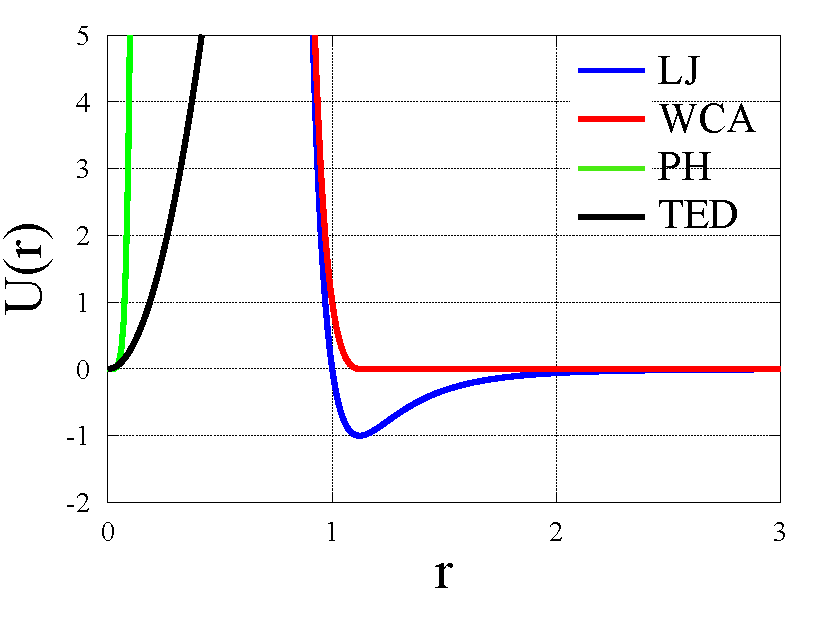
\includegraphics[width=100mm]{rysunki/potencjaly.pdf}
\caption{Porównanie potencjałów LJ, WCA, PH oraz TED.}
\label{potencjaly}
\end{figure}
\\
{Potencjał Lennarda-Jonesa} ma postać,
\begin{equation}
\phi_{LJ}(\underline{r}_{ij})=4 \epsilon \left[ \left( \sigma \over \underline{r}_{ij} \right)^{12} - \left( \sigma \over \underline{r}_{ij} \right)^{6} \right],
\end{equation}
gdzie $\underline{r}_{ij}$ to odległość pomiędzy dwiema cząsteczkami $i, j$, $\sigma$ to średnica jednej cząsteczki, natomiast $\epsilon$ stanowi parametr skalowania energii. Potencjał Lennarda-Jonesa może dobrze modelować oddziaływania między atomami gazów szlachetnych. W pracy zazwyczaj wartości $\sigma$ oraz $\epsilon$ były dobrane zgodnie z wynikami badań eksperymentalnych dla atomów argonu, czyli $\sigma = 3.405 A$ oraz $\epsilon=120 K$ \cite{Rahman}. Oddziaływanie typu LJ szybko zbiega do zera wraz z rosnącą odległością między cząsteczkami. Celem przyspieszenia numerycznych obliczeń, można wykorzystać ten fakt i dokonać tak zwanego odcięcia potencjału, tzn. przyjąć, że dla odległości między cząsteczkami większymi niż dystans odcięcia, wartość oddziaływania jest równa zeru. Potencjał {Weeks - Chandler - Andersen} definiuje się w oparciu o potencjał LJ. Ma on następującą postać,
\begin{equation}
\phi_{WCA}(r_{ij})= \begin{cases} 4 \epsilon \left[ \left( \sigma \over r_{ij} \right)^{12} - \left( \sigma \over r_{ij} \right)^{6} \right]+1 & \mbox{dla } r_{ij}<2^{1/6},  \\ 0 & \mbox{dla } r_{ij}>2^{1/6}. \end{cases}
\end{equation}
Potencjał WCA jest konstruowany z potencjału Lennarda-Jonesa poprzez odcięcie w~minimum $r_{cut}=r_{min}=2^{1/6}\sigma$ i przesunięcie o $\epsilon$. Posiada tylko część odpychającą. Jest~potencjałem krótkozasięgowym o ciągłej pochodnej w punkcie odcięcia $r_{cut}$. Z tego powodu potencjał WCA jest często wykorzystywany do obliczeń testowych. Dodatkowo, jest on referencyjnym potencjałem w zaburzeniowej teorii cieczy. 
Potencjałem służącym wiązaniu cząsteczek ścian do punktów wirtualnej sieci krystalicznej może być anharmoniczny potencjał stosowany przez Pertavic i Harowella {PH} w pracach \cite{Petravic2005, PetravicHarrowell2006}. Ma on postać,
\begin{equation}
\phi_{T}(\underline{r}_i)=k_4 [\underline{r}_i - \underline{r}_{0,i}]^4 + k_6 [\underline{r}_i - \underline{r}_{0,i}]^6,
\end{equation}
gdzie $\underline{r}_i$ jest chwilowym wektorem położenia $i$-tej cząsteczki ściany, natomiast $\underline{r}_{0,i}$ jest położeniem $i$-tego węzła wirtualnej sieci krystalicznej. Stałe $k_4$ oraz $k_6$ wynoszą odpowiednio $k_4=5 \times 10^3$ i $k_6=5 \times 10^6$. Celem powyższego potencjału jednocząsteczkowego jest utrzymanie atomów sieci w ramach jednego bloku oraz zapobieżenie dyfuzji cząsteczek ograniczonej części do wnętrza ścian. Dobrane współczynniki zapewniają anharmoniczne wahania cząsteczek ścian wokół węzłów wirtualnej sieci na dystans nie większy niż $10\%$ stałej sieciowej. Atomy mogą być wiązane do punktów sieci krystalicznej również za pomocą potencjału harmonicznego. Przykładem może być potencjał zastosowany w~pracy \cite{Todd} przez Todda, Evansa i Daivisa {TED}, którego postać,
\begin{equation}
\phi_{T}(\underline{r}_i)=k_2 [\underline{r}_i - \underline{r}_{0,i}]^2,
\end{equation}
gdzie $k_2=57.15$.
Omówione potencjały przedstawia rysunek \ref{potencjaly}. 
%
\section{Konwencja jednostek zredukowanych}
\label{redunit}
%
Wykonane obliczenia przedstawia się korzystając z układu jednostek SI oraz z układu jednostek zredukowanych. Konwencja jednostek zredukowanych polega na wyrażaniu wielkości fizycznych w jednostkach charakterystycznych dla oddziaływania w układzie. W odniesieniu do oddziaływań typu LJ są to średnica atomu $\sigma$ oraz głębokość studni oddziaływania $\epsilon$. Załóżmy, że interesują nas jednostki odpowiadające oddziaływaniu pomiędzy atomami argonu. Związek zastosowanych jednostek z układem jednostek SI jest następujący: \\
\\
{a) jednostka energii:} $\epsilon/k_B = 120$ [K], $\epsilon = 1.656 \cdot 10^{-21}$ [J],\\
{b) jednostka masy:} $m=39.95$ [u]$=66.317 \cdot 10^{-27}$ [kg], \\
{c) jednostka odległości:} $\sigma=0.34$ [nm]$ = 0.34 \cdot 10^{-9}$ [m],\\
{d) jednostka czasu:} $\tau = \sigma \sqrt{m/\epsilon} = 2.15$ [ps]$ = 2.5 \cdot 10^{-12}$ [s], \\
{e) jednostka prędkości:} $v=v^{*} \cdot {\sigma / \tau} = v^{*} \cdot 158$ [m/s], \\
{f) jednostka ciśnienia:} $P=P^{*} \cdot \epsilon / \sigma^{3} = P^{*} \cdot 42.133$ [MPa].
%
\section{Algorytmy numerycznego całkowania \\ równań różniczkowych}
\label{algolnum}
Rozwiązywanie układów równań różniczkowych zwyczajnych (do których należą stosowane w Dynamice Molekularnej) polega na zastosowaniu numerycznych metod małych kroków czasowych. Idea numerycznego rozwiązywania równań ruchu polega na zamianie równań różniczkowych na równania różnicowe. W praktyce symulacji MD szczególną rolę odgrywają algorytmy z rodziny algorytmów Verleta \cite{Verlet1, Verlet2} i Rungego-Kutty \cite{AllenTildesley}. Algorytm Verleta w swojej podstawowej formie opiera się na rozwinięciu równania ruchu w szereg Taylora wokół chwili początkowej $t$ do chwili $t+\Delta t$ oraz chwili $t-\Delta t$. Następnie uzyskane rozwinięcia odejmuje się stronami, redukując tym sposobem kolejne parzyste człony. W praktyce uzyskane równanie ogranicza się do członów czwartego rzędu. Można powiedzieć, że Algorytm Verleta opiera się na ekstrapolacji - nowe położenie wyznacza się w oparciu o znajomość położenia aktualnego i przeszłego. Ważną cechą algorytmu Verleta jest to, że wymaga on obliczania siły między cząsteczkami tylko raz w~danym cyklu, dzięki czemu jest stosunkowo szybkim algorytmem (obliczanie sił między cząsteczkami wymaga zastosowania podwójnej pętli, która często pochłania $80-90 \%$ czasu trwania cyklu obliczeń). Poniżej przedstawione zostały najważniejsze warianty algorytmu Verleta, a więc wersja "podstawowa", "prędkościowa" oraz "skaczącej żaby".\\
\textbf{Wariant podstawowy:}\\
rozwijając równanie ruchu postaci $\underline{F}=m \cdot d^2 \underline{r} / dt^2$ w szereg Taylora, otrzymujemy
\begin{equation}
\underline{r}(t+\Delta t) = \underline{r}(t)+ \frac{d \underline{r}(t)}{dt} \Delta t + \frac{1}{2} \frac{d^2 \underline{r}(t)}{dt^2} (\Delta t)^2 + \frac{1}{6} \frac{d^3 \underline{r}(t)}{dt^3} (\Delta t)^3 + O(\Delta t)^4,
\end{equation}
\begin{equation}
\underline{r}(t-\Delta t) = \underline{r}(t) - \frac{d \underline{r}(t)}{dt} \Delta t + \frac{1}{2} \frac{d^2 \underline{r}(t)}{dt^2} (\Delta t)^2 - \frac{1}{6} \frac{d^3 \underline{r}(t)}{dt^3} (\Delta t)^3 + O(\Delta t)^4.
\end{equation}
Dodając powyższe równania stronami otrzymujemy wyrażenie na położenie cząsteczki w czasie $t+\Delta t$
\begin{equation}
\underline{r}(t+\Delta t)= 2 \underline{r}(t) - \underline{r}(t-\Delta t) + \frac{\underline{F}(t)}{m}(\Delta t)^2.
\end{equation}
Prędkość można obliczyć jako
\begin{equation}
\underline{v}(t)=\frac{\underline{r}(t+\Delta t)-\underline{r}(t-\Delta t)}{2 \Delta t}.
\end{equation}
\textbf{Wariant prędkościowy:} \\
ta zmodyfikowana wersja algorytmu Verleta jest wyrażona poprzez następujący zestaw równań
\begin{equation}
\underline{r}(t+\Delta t)=\underline{r}(t)+\underline{v}(t)\Delta t + \frac{1}{2} \frac{\underline{F}(t)}{m}(\Delta t)^2,
\end{equation}
\begin{equation}
\underline{v}(t+\Delta t/2)=\underline{v}(t) + \frac{1}{2} \frac{\underline{F}(t)}{m}(\Delta t),
\end{equation}
\begin{equation}
\underline{F}(t+\Delta t)=-\nabla U (\underline{r}(t+\Delta t)),
\end{equation}
\begin{equation}
\underline{v}(t+\Delta)=\underline{v}(t+\Delta t/2) + \frac{1}{2} \frac{\underline{F}(t+\Delta t)}{m}(\Delta t).
\end{equation}
Ważną cechą tego algorytmu jest fakt, że położenia i prędkości są wyliczane dokładnie w~tym samym kroku czasowym (co może być istotne z punktu widzenia równań termostatu Nos\'{e}go-Hoovera).
\\
\textbf{Wariant skaczącej żaby:}\\
algorytmem najczęściej stosowanym w trakcie prowadzonych badań był wariant "skaczącej żaby"(\textit{ang.} leap frog). Wyraża go następujący układ równań
\begin{equation}
\underline{r}(t+\Delta t) = \underline{r} (t) + \underline{v}(t+\Delta t/2)\Delta t,
\end{equation}
\begin{equation}
\underline{v}(t+\Delta t/2)=\underline{v}(t-\Delta t/2)+\frac{\underline{F}(t)}{m}(\Delta t),
\end{equation}
\begin{equation}
\underline{v}(t)=\frac{1}{2} \left( \underline{v}(t-\Delta t/2) + \underline{v}(t+\Delta t/2) \right).
\end{equation}
Wszystkie warianty algorytmu Verleta są równoważne sobie, ale różnią się propagacją błędów zaokrągleń. Są zaliczane do algorytmów o dokładności globalnej rzędu drugiego.
\\
Drugą rodziną algorytmów stosowanych w symulacjach jest rodzina algorytmów Rungego-Kutty (RK). Ze względu na swoją dokładność, często stosowanym jest algorytm czwartego rzędu (RK4). W porównaniu do algorytmów Verleta, algorytm RK4 cechuje większa dokładność. Zastosowanie algorytmu RK4 wymaga znajomości początkowych położeń i prędkości oraz pozwala wyznaczać je w tym samym kroku czasowym $t+\Delta t$. Jego wadą jest konieczność czterokrotnego obliczania sił między cząsteczkami w każdym cyklu, co znacznie spowalnia symulację. Schemat wyznaczania kolejnej wartości rozwiązania równania różniczkowego postaci $\dot{y}=f(x,y)$, przy znajomości wartości początkowej $y(x_0)=y_0$ przedstawia poniższy zestaw równań.
\begin{equation}
y_{n+1} = y_n + 1/6 (k_1 + 2k_2 + 2k_3 + k_4),
\end{equation}
gdzie
\begin{equation}
\begin{gathered}
k_1=f(x_n, y_n)\Delta t,\\
%
k_2=f(x_n+\Delta t/2,y_n+1/2 k_1 \Delta t)\Delta t,\\
%
k_3=f(x_n+\Delta t/2,y_n+1/2 k_2 \Delta t)\Delta t,\\
%
k_4=f(x_n+\Delta t,y_n+ k_3 \Delta t)\Delta t.
\end{gathered}
\end{equation}
 
%
\section{Warunki brzegowe}
\label{warbrzeg}
%
W metodzie MD wielkości fizyczne są otrzymywane jako średnie po czasie z trajektorii fazowej układu. Liczba cząsteczek w symulacjach MD jest stosunkowo niewielka w~odniesieniu do liczby Avogadra $N_A=6.022140857 \cdot 10^{23}$. Aby zmniejszyć wpływ ograniczonej liczby cząsteczek oraz brzegów układu wprowadza się tzw. periodyczne warunki brzegowe. Dzięki zastosowaniu periodycznych warunków brzegowych obliczane wielkości średnie są bliskie wartościom termodynamicznym już dla stosunkowo małej liczby $N$, ponieważ dla wielu wielkości fizycznych $A_{\infty} = A_N + \frac{a}{N^\alpha}$, gdzie $A$ to wartość pewnej wielkości fizycznej, $A_{\infty}$ to jej wartość w granicy termodynamicznej, $N$ oznacza liczbę cząsteczek w układzie, $A_{N}$ wartość wielkości fizycznej w układzie złożonym z $N$ cząsteczek, natomiast $a$ i $\alpha$ to pewne stałe. 
\\
\\
W pracy periodyczne warunki brzegowe zastosowano w kierunkach planarnych $x$ i $y$. W tych kierunkach zastosowano również konwencję najbliższego obrazu. W kierunku $z$ nie zastosowano periodycznych warunków brzegowych - układ był ograniczony przez ściany. W związku z tym, periodyczne warunki brzegowe zastosowane w układzie, można zapisać jako,
\begin{equation}
\begin{gathered}
x_i=x_i-L \cdot round (x_i / L), \\
y_i=y_i-L \cdot round (y_i / L),
\end{gathered}
\end{equation}
gdzie $L$ oznacza rozmiar krawędzi komórki symulacyjnej zarówno w kierunku $x$ i $y$. Zastosowane periodyczne warunki brzegowe w płaszczyźnie $xy$ ilustruje rysunek \ref{period_war_brz}.
\begin{figure}[h]
\centering
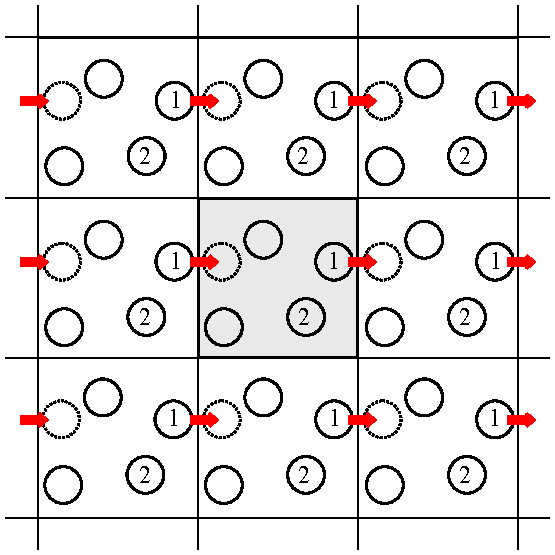
\includegraphics[width=80mm]{rysunki/PBC.pdf}
\caption{Ilustracja periodycznych warunków brzegowych 2D.}
\label{period_war_brz}
\end{figure}
Środkowa część przedstawia komórkę symulacyjną. Jest~ona~otoczona przez układ wirtualnych komórek, zawierających dokładnie te same cząsteczki (ich kopie), w tych samych położeniach (względem własnego układu współrzędnych wirtualnej komórki). Cząsteczka przekraczając granicę obszaru symulacji pojawia się po jego przeciwległej stronie, ponieważ zastępuje ją jej wchodząca kopia.
%
\section{Nierównowagowa dynamika molekularna (NEMD)}
%
Klasycznym przykładem schematu NEMD jest stosowany w układach objętościowych dla przepływu Couette algorytm SLLOD \cite{EvansMoris1990} z warunkami brzegowymi Lees-Edwards (rysunek \ref{period_war_brz_LE}). Algorytm pozwala wytworzyć stan stacjonarny o liniowym profilu prędkości. Oryginalny wariant algorytmu SLLOD ma postać,
\begin{equation}
\begin{gathered}
\underline{\dot{r}}_i=\frac{\underline{p}_i}{m_i}+\gamma r_{yi} \underline{\hat{x}}, \\
\underline{\dot{p}}_i=\underline{F}_i -\gamma p_{yi} \underline{\hat{x}} - \alpha\underline{p}_i, \\
\alpha=\frac{\sum_i^N \underline{F}_i \cdot \underline{p}_i}{\sum_i^N \underline{p}_i^2},
\end{gathered}
\end{equation}   
%
gdzie wyrazy $+\gamma r_{yi} \underline{\hat{x}}$, $-\gamma p_{yi} \underline{\hat{x}}$ wprowadzają liniowy profil prędkości cząsteczek w układzie, $\gamma$ jest prędkością ścinania, a $\alpha$ jest zmienną związaną z zastosowanym termostatem (w przypadku powyższych równań zastosowano termostat gaussowski).
\begin{figure}[h]
\centering
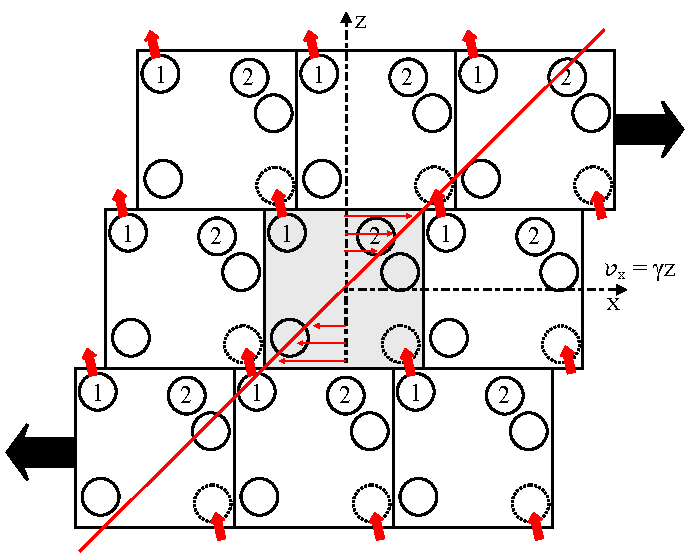
\includegraphics[width=90mm]{rysunki/PBC_LE.pdf}
\caption{Ilustracja periodycznych warunków brzegowych Lee-Edwards w przestrzeni dwuwymiarowej oraz przepływu Couette. Środkowy kwadrat reprezentuje komórkę symulacyjną. Dolna część płynu przemieszcza się w przeciwnym kierunku niż górna (zgodnie z czarnymi strzałkami). Repliki komórki symulacyjnej przemieszczają się w kierunkach zgodnych z przepływem.}
\label{period_war_brz_LE}
\end{figure}

\section{Schemat blokowy programu}
%
Elementy typowego programu MD przedstawiono w postaci schematu blokowego na rysunku \ref{schemat_blokowy}. 
\begin{figure}[h]
\centering
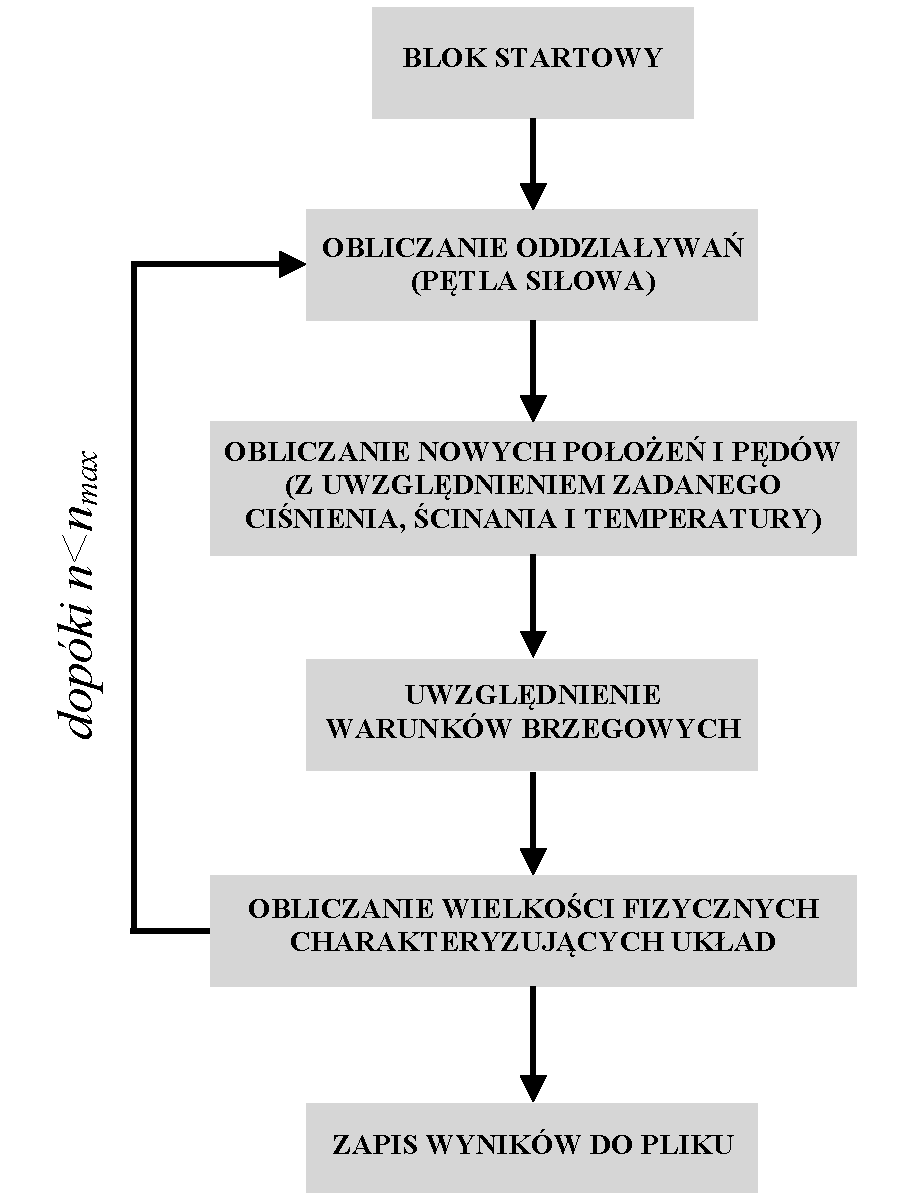
\includegraphics[width=80mm]{rysunki/schemat_blokowy.pdf}
\caption{Schemat blokowy programu symulacji MD.}
\label{schemat_blokowy}
\end{figure}
W bloku startowym inicjowane są zmienne opisujące stan układu oraz początkowe położenia i prędkości cząsteczek. W bloku oddziaływań obliczane są siły działające na poszczególne cząsteczki. Ta część programu pochłania najwięcej czasu, ponieważ w jednym cyklu należy wykonać $N^2$ operacji związanych z dwucząsteczkowymi oddziaływaniami w układzie. Aby przyspieszyć obliczenia stosuje się określone rozwiązania:
\begin{itemize}
\item{odcięcie potencjału - oddziaływanie między cząsteczkami jest obliczane tylko wówczas, gdy odległość między nimi nie przekracza dystansu odcięcia,}
\item{lista Verleta - każdej cząsteczce przyporządkowana jest lista najbliższych sąsiadów i tylko z tymi cząsteczkami są obliczane oddziaływania. Sama lista jest aktualizowana co stałą liczbę kroków lub gdy którakolwiek cząsteczka pokona zadany dystans, }\\
\\
\item{struktura komórkowa - komórka symulacyjna jest dzielona na podobszary i oddziaływania w każdym z nich są liczone oddzielnie i tylko dla cząsteczek zawartych w danej podkomórce i sąsiadujących podkomórkach \cite{AllenTildesley}. }
\end{itemize}
Po wyliczeniu sił działających na cząsteczki, odbywa się wyznaczenie nowych położeń i~prędkości (dla czasu $t+\Delta t$) korzystając z algorytmów numerycznego całkowania równań różniczkowych. Ponieważ nowe położenie cząsteczki może znajdować się poza obszarem komórki symulacyjnej, należy po ich uzyskaniu zastosować warunki brzegowe, tzn. wykonać procedurę opisaną w części \ref{warbrzeg}. Następnie wykonywane są obliczenia wielkości fizycznych takich jak temperatura, ciśnienie, współczynnik tarcia, itd. Jeżeli aktualny krok ma w kolejności indeks mniejszy niż liczba założonych kroków symulacji $n_{max}$ dochodzi do powtórzenia cyklu od ponownego wykonania pętli siłowej. Po wykonaniu wszystkich cykli, uzyskane wyniki są zapisywane do pliku.
%
%
\begin{thebibliography}{3}
%
\begin{spacing}{1.0}

\bibitem{Rugh1997} H.H. Rugh, Phys. Rev. Lett. {\bf 78}, 772 (1997).

\bibitem{Jepps2000} O.G. Jepps, G. Ayton, and D.J. Evans, Phys. Rev. E {\bf 62}, 4757 (2000).

\bibitem{Rickayzen2001} G. Rickayzen and J.G. Powles, J. Chem. Phys. {\bf 114} 4333 (2001).

\bibitem{TravisBraga2005} C. Braga, K.P. Travis, J. Chem. Phys. {\bf 123}, 134101 (2005).

\bibitem{TravisBraga2006} C. Braga and K. P. Travis, J. Chem. Phys. {\bf 124}, 104102 (2006).

\bibitem{Hoover2009} Wm. G. Hoover and C. G. Hoover, Phys. Rev. E {\bf 79}, 046705, (2009)

\bibitem{Pieprzyk2015} S. Pieprzyk, D. M. Heyes, Sz. Maćkowiak, and A. C. Brańka, Phys. Rev. E {\bf 91}, 033312 (2015)

\bibitem{Landau} L. Landau, E. Lifszyc, {\it Mechanika}, (PWN, Warszawa, 1965).

\bibitem{Zubariew} D. N. Zubariew, {\it Termodynamika Statystyczna}, (PWN, Warszawa, 1974).

\bibitem{Todd} B. D. Todd, D. J. Evans, P. J. Daivis, Phys. Rev. E {\bf 52}, 1627 (1995).

\bibitem{Petravic2005} J. Petravic, P. Harrowell PRE {\bf 71}, 061201 (2005).

\bibitem{PetravicHarrowell2006} J. Petravic, P. Harrowell, J. Chem. Phys. {\bf 124}, 014103 (2006).

\bibitem{Rahman} A. Rahman, Physical Review {\bf 136}, A405 (1964).

\bibitem{Verlet1} L. Verlet, Phys. Rev. {\bf 159}, 98 (1967).
\bibitem{Verlet2} L. Verlet, Phys. Rev. {\bf 165}, 201 (1967).

\bibitem{AllenTildesley} M.P. Allen, D.J. Tildesley, {\it Computer Simulation of Liquids}, \\(Oxford University Press, New York, 1989).

\bibitem{EvansMoris1990} D. J. Evans, G. Morriss, {\it Statistical Mechanics of Nonequilibrium Liquids}, \\(Cambridge University Press, Cambridge, 2008).


\end{spacing}
%
%
%KONIEC REFERENCJI ZE WSTEPU



\end{thebibliography}
\end{document}

  


